\documentclass[11pt,a4paper,DIV=12]{scrartcl}
\usepackage[utf8]{inputenc}
\usepackage[T1]{fontenc}
\usepackage[english]{babel}
\usepackage[hidelinks]{hyperref}
\usepackage{framed}
\usepackage{color}
\usepackage{enumitem}
\usepackage{amsmath}
\usepackage{amsfonts}
\usepackage{amssymb}
\usepackage{trfsigns}
\usepackage{graphicx}
\usepackage{subfig}
\newcommand{\red}{\textcolor{red}}
\usepackage{comment}
\specialcomment{Loesung}{\begin{framed}\noindent}{\end{framed}\noindent}
%\excludecomment{Loesung}


\begin{document}
{\raggedleft Sascha Spors\\
Professorship Signal Theory and Digital Signal Processing\\
Institute of Communications Engineering (INT)\\
Faculty of Computer Science and Electrical Engineering (IEF)\\
University of Rostock, Germany\\}
\vspace{0.5cm}
\noindent This tutorial is provided as Open Educational Resource, to be found at\\
\url{https://github.com/spatialaudio/digital-signal-processing-exercises}\\
accompanying the DSP lecture\\
\url{https://github.com/spatialaudio/digital-signal-processing-lecture}\\
Both are licensed under the Creative Commons Attribution 4.0 International
License for text/graphics and under the MIT License for software. Please
attribute this work as \textit{Frank Schultz, Digital Signal Processing - A
Tutorial Featuring Computational Examples} with the github URL.
\newline

\textbf{Digital Signal Processing Tutorial 1 \& 2, Winter Semester 2019/20}
(Course \#24505)
authors: Frank Schultz (concept, initial draft, OER ready),
Vera Erbes (proof reading and validation, translation from German to English)\\
Feel free to contact frank.schultz@uni-rostock.de.

%------------------------------------------------------------------------------
\section*{\underline{Spectral Analysis of Deterministic Signals}}
\renewcommand{\contentsname}{}
\tableofcontents
\vspace{.7cm}

\clearpage
\section{DFT}
Why just another DFT tutorial? Well, this is a collection of calculus,
graphs and exercises that the authors found most useful for teaching purposes
in the last decade.
The graphs and the didactical approach following \cite{Moeser2011} might be
a way of DFT storytelling that is rarely found in classic textbooks
and deserve survival.

% ---------------------------------------------------------------------------------
\subsection{DFT Definitions}
The discrete Fourier transform (DFT, often interpreted as signal analysis) and
its counterpart the inverse DFT (IDFT, often interpreted as signal synthesis)
are defined as \cite[eq.~(8.11) and (8.12)]{Oppenheim2010}
\begin{equation}
X[\mu]=\sum_{k=0}^{N-1}x[k]\cdot W_N^{k\mu} \hspace{2cm}
x[k]=\frac{1}{N}\sum_{\mu=0}^{N-1}X[\mu]\cdot W_N^{-k\mu}
\end{equation}
using the so-called twiddle factor or DFT kernel
\begin{equation}
W_N=\e^{-\im\frac{2\pi}{N}}
\end{equation}
relating an $N$ samples discrete-time signal $x[k]$ and its $N$ coefficients
(also called bins) discrete-frequency DFT spectrum $X[\mu]$.
%
In general, the DFT/IDFT supports $x[k]\in \mathbb{C}$ and
$X[\mu]\in \mathbb{C}$.
%
Later, some useful relations will be obtained when assuming
$x[k]\in\mathbb{R}$.

In the literature, the DFT/IDFT pair may be differently defined, such as e.g.
\begin{align}
&X[\mu]=\underbrace{{\frac{1}{N}}}_{K_\text{DFT}}\sum_{n=0}^{N-1}x[k]\cdot W_N^{k\mu}
\,\laplace\hspace{2cm}
x[k]=\underbrace{{1}}_{K_\text{IDFT}}\cdot\sum_{\mu=0}^{N-1}X[\mu]\cdot W_N^{-k\mu}\\
&X[\mu]=\underbrace{{\frac{1}{\sqrt{N}}}}_{K_\text{DFT}}\sum_{n=0}^{N-1}x[k]\cdot W_N^{k\mu}
\,\laplace\hspace{2cm}
x[k]=\underbrace{{\frac{1}{\sqrt{N}}}}_{K_\text{IDFT}}\sum_{\mu=0}^{N-1}X[\mu]\cdot W_N^{-k\mu},
\label{eq:orthonorm}
\end{align}
where different normalisation schemes are applied.
%
However, a valid DFT/IDFT-pair must always fulfill
\begin{align}
K=K_{\text{IDFT}}\cdot K_{\text{DFT}}=\frac{1}{N},
\end{align}
so that
\begin{align}
x[k]&=\text{IDFT}\left\{\text{DFT}\left\{x[k]\right\}\right\}
\label{eq:x_idft_dft_x}
\\
X[\mu]&=\text{DFT}\left\{\text{IDFT}\left\{X[\mu]\right\}\right\}
\label{eq:X_dft_idft_X}
\end{align}
holds.
%
Hence, either $K_{\text{IDFT}}$ or $K_{\text{DFT}}$ can be chosen according to
the specific application and then the other parameter is determined by $K$.
%
Another convention is related to the sign of exp() in the twiddle factor.
%
This may also be defined as
\begin{equation}
W_N=\e^{\red{+}\im\frac{2\pi}{N}}
\end{equation}
if required for specific applications.
%
Note that the DFT/IDFT equations do not care about signal interpretation, they
transform a vector to another vector.
%
The general definition of the DFT/IDFT-pair is thus given as
\begin{equation}
X[\mu]=K_\text{DFT}\sum_{k=0}^{N-1}x[k]\cdot W_N^{\pm k\mu}
\hspace{2cm}
x[k]=K_\text{IDFT}\sum_{\mu=0}^{N-1}X[\mu]\cdot W_N^{\mp k\mu}
\end{equation}
using
\begin{equation}
W_N=\e^{-\im\frac{2\pi}{N}},
\hspace{1cm}
K_\text{IDFT}\cdot K_\text{DFT}=\frac{1}{N}.
\end{equation}
%
In the majority of DSP-related books and software the DFT/IDFT pair is defined
as
\begin{align}
X[\mu]=&\sum_{k=0}^{N-1}x[k]\cdot\e^{-\im\frac{2\pi}{N}k\mu}
\hspace{0.5cm}
\text{Python numpy \texttt{X=np.fft.fft(x)}, Matlab: \texttt{X=fft(x)}}
\label{eq:DFT}\\
x[k]=\frac{1}{N}&\sum_{\mu=0}^{N-1}X[\mu]\cdot\e^{+\im\frac{2\pi}{N}k\mu}
\hspace{0.4cm}
\text{Python numpy \texttt{x=np.fft.ifft(X)}, Matlab: \texttt{x=ifft(X)}}
\label{eq:IDFT}
\end{align}
which will also be used throughout the lecture and the tutorial.
%
This convention implies that positive constant group delays in the DFT spectrum
$X$ are interpreted as causal signal delays for $x$.

The discrete-time Fourier transform (DTFT) pair
\begin{align}
X(\Omega)=&\sum_{k=-\infty}^\infty x[k]\cdot\e^{-\im\Omega k}
\label{eq:DTFT}\\
x[k]=\frac{1}{2\pi}&\int\limits_{-\pi}^\pi X(\Omega)\cdot\e^{+\im\Omega k}\text{d}\Omega.
\end{align}
is defined with the same signs in the exp() and the prefactor $\frac{1}{2\pi}$
belonging to the synthesis equation in the same way as for the used definition
of the DFT pair.

% -----------------------------------------------------------------------------
\subsection{Matrix Notation and Use of Linear Algebra Fundamentals}
The DFT is a classic application for a fundamental linear algebra problem, i.e.
solving a set of linear equations, or in another train of thought: transferring
one vector to another vector in hope for more convenient data representation,
such as here for spectrum analysis.
%
And of course it is not pure hope which helps us, but the appropriate choice
of a vector base that (approximately) solves our problem.
%
It is thus worth to grasp these links for an in-depth understanding.

The DFT of length $N$ is a brilliant example for a special base of orthogonal
vectors that are set up from the roots of the $z^N=1$ equation, i.e.
equiangularly distributed locations along the unit circle within the complex
plane, cf. Fig.~\ref{DFT_Eigenfrequenzen_N4_N5}.
%
To build these vectors, let us recall the twiddle factor
\begin{equation}
W=\e^{-\im\frac{2\pi}{N}},
\end{equation}
here omitting the $N$ subscript to avoid confusion with the following subscripts
that indicate matrix and vector dimensions.
%
Now, by inspecting the DFT analysis equation \eqref{eq:DFT} one might figure
what pairs of $k$ and $\mu$ are required and bring them into a certain sequence,
namely putting them into an appropriate matrix.
%
This so called DFT matrix $\mathbf{W}_{N \times N}$ can be built from the
outer product (note the symmetry)
\begin{equation*}
\mathbf{A}_{N \times N} =
\begin{bmatrix}
0\\
1\\
2\\
3\\
\vdots\\
N-1
\end{bmatrix}
\cdot
\begin{bmatrix}
0 & 1 & 2 & 3 &\cdots & N-1
\end{bmatrix}
=
\begin{bmatrix}
0 & 0 & 0 & 0 & \cdots & 0\\
0 & 1 & 2 & 3 & \cdots & (N-1)\\
0 & 2 & 4 & 6 & \cdots & 2(N-1)\\
0 & 3 & 6 & 9 & \cdots & 3(N-1)\\
\vdots & & \cdots& & & \vdots\\
0 & (N-1) & 2(N-1) & 3(N-1) & \cdots & (N-1)^2
\end{bmatrix}
\end{equation*}
%
applying it to the twiddle factor by element-wise operation
%
\begin{equation}
\mathbf{W}_{N \times N} =
(\e^{-\im\frac{2\pi}{N}})^\mathbf{A} =
\e^{-\im\frac{2\pi}{N} \mathbf{A}}.
\end{equation}
%
The reader might verify that this matrix is orthogonal
(note that the complex dot product is required here).
%
Then, the DFT \eqref{eq:DFT} can be written in matrix notation as
\begin{equation}
\begin{bmatrix}
X[\mu=0]\\
X[\mu=1]\\
X[\mu=2]\\
\vdots\\
X[\mu=N-1]
\end{bmatrix}
=
\begin{bmatrix}
W^{0 \cdot 0} & W^{0 \cdot 1} & W^{0 \cdot 2} & \cdots & W^{0 \cdot (N-1)}\\
W^{1 \cdot 0} & W^{1 \cdot 1} & W^{1 \cdot 2} & \cdots & W^{1 \cdot (N-1)}\\
W^{2 \cdot 0} & W^{2 \cdot 1} & W^{2 \cdot 2} & \cdots & W^{2 \cdot (N-1)}\\
\vdots & & \cdots& & \vdots\\
W^{(N-1) \cdot 0} & W^{(N-1) \cdot 1} & W^{(N-1) \cdot 2} & \cdots & W^{(N-1)(N-1)}\\
\end{bmatrix} \,
\begin{bmatrix}
x[k=0]\\
x[k=1]\\
x[k=2]\\
\vdots\\
x[k=N-1]
\end{bmatrix},
\end{equation}
shortly as
\begin{equation}
\mathbf{X}_{N \times 1} = \mathbf{W}_{N \times N} \, \mathbf{x}_{N \times 1}.
\end{equation}
Note that linear algebra typical notates matrices with uppercase letters and vectors
with lowercase letters. Common signal processing convention uses lowercase letters for
signals and uppercase letters for spectrum. Following the latter $\mathbf{X}$ is
not a matrix, but a vector containing the DFT spectrum.

The inverse of the DFT matrix reads
\begin{equation}
\mathbf{W}^{-1}
= \frac{1}{N} \mathbf{W}^\mathrm{H}
= \frac{1}{N} \mathbf{W}^\mathrm{*},
\end{equation}
with
$^\mathrm{H}$ denoting conjugate-complex and transpose operation.
This constitutes a special case for complex valued, symmetric matrix $\mathbf{W}$.
%
Since $\mathbf{W}$ is also square, no transpose is required, but only the
conjugate complex operation $()^*$, which is just the sign reversal
in the exp() of twiddle factor.
%
If the matrices are normalized, such that
\begin{equation}
(\frac{1}{\sqrt{N}} \mathbf{W}^\mathrm{H}) \, (\frac{1}{\sqrt{N}} \mathbf{W}) = \mathbf{I}
\end{equation}
then they are unitary, i.e. the complex conjugate transpose of the complex
square matrix is at the same time the inverse.
This is a key feature for DFT.

The IDFT is then solving the set of equations
$\mathbf{X} = \mathbf{W} \mathbf{x}$ for a given $\mathbf{X}$ and an unknown $\mathbf{x}$
via
\begin{equation}
\mathbf{x} = \mathbf{W}^{-1} \mathbf{X} = \frac{1}{N}\mathbf{W}^* \mathbf{X}
\end{equation}
which precisely corresponds to \eqref{eq:IDFT}.
Furthermore, analysis (DFT) and subsequent synthesis (IDFT) yields the input
vector again, such as
\begin{equation}
\mathbf{x} = \frac{1}{N}\mathbf{W}^* \, (\mathbf{W} \mathbf{x}) =
(\frac{1}{N}\mathbf{W}^* \, \mathbf{W}) \mathbf{x} = \mathbf{x},
\end{equation}
due to $\frac{1}{N}\mathbf{W}^* \mathbf{W} = \mathbf{I}$.
This is identical to the statement \eqref{eq:x_idft_dft_x}.

The reader might verify that the following DFT/IDFT pairs with $N=4$ pairs hold.
%
The input vector $\mathbf{x}=[1,1,1,1]^\mathrm{T}$ (pure DC component)
yields $\mathbf{X} = [4,0,0,0]^\mathrm{T}$ (energy only at 'zero'-th frequency).
The spectrum $\mathbf{X} = [1,1,1,1]^\mathrm{T}$ (all frequencies exhibit equal
energy) yields $\mathbf{x} = [1,0,0,0]^\mathrm{T}$ (the discrete Dirac impulse).

%------------------------------------------------------------------------------
\subsection{FFT as a Fast Calculation of the DFT}
The DFT/IDFT equations include redundant calculation steps due to the twiddle
factor characteristics.
%
A straightforward implementation for large $N$ demands very high computing load.
%
For example, most obviously the same $W_N^{k\mu}$ is derived for $\mu=1$, $k=2$
and $\mu=2$, $k=1$, cf. the entries of the matrices $\mathbf{A}$ and $\mathbf{W}$.
%
For large $N$, many angles $\frac{2\pi}{N}k\mu$ are equivalent.
%
This is exemplarily shown in Fig.~\ref{Twiddle1}, Fig.~\ref{Twiddle2} and
Fig.~\ref{Twiddle3} for $N=8$, $N=9$ and $N=48$ DFTs.
%
These plots indicate certain symmetries, which is to be expected since the
underlying matrix has symmetry as well.

Algorithms that make use of these symmetries in order to reduce or simplify
computation steps are subsumed as Fast Fourier Transform (FFT).
%
Explained in a sloppy way, FFTs calculate certain repeatedly used twiddle factor
results only once.
%
The first proposed FFT algorithm is from Cooley and Tukey \cite{Cooley1965},
that relies on $N=2^m$, $m\in\mathbb{N}$.
%
Nowadays, many other and improved FFT algorithms exist, so that if $N$
is accessible for a prime factorisation, an FFT can be calculated with much less
processing load than a DFT.
%
In fact, the invention of fast calculation of the DFT is a (if not the)
milestone in DSP making these huge technological steps in the last decades of the
digital age.

The FFT concept can be derived from the linear algebra problem finding a
suitable factorization for $\mathbf{W}$ that involves sparse matrices and plain
vector permutations (which not need to be calculated as matrix operations) and
thus reduces multiplications/additions.
%
You will reinvent this basis concept in one of the homework assignments.


\begin{figure}[t]
		\centering
		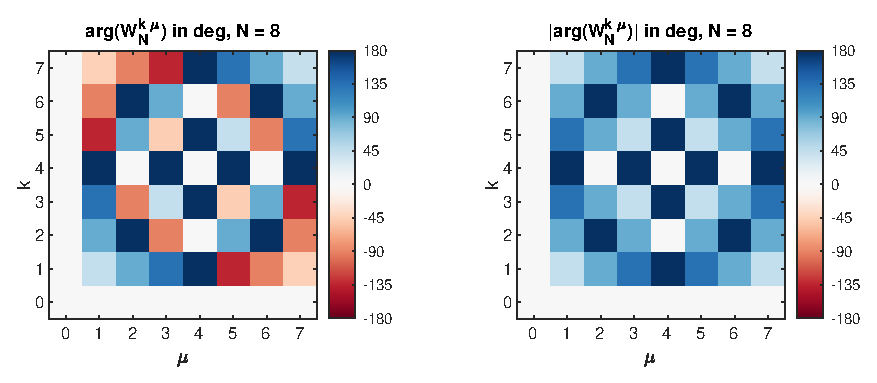
\includegraphics[]{graphics/TwiddleFactorMatrix_N8}
		\caption{$\text{arg}(W_N^{\mu k})$ (left) and $|\text{arg}(W_N^{\mu k})|$
		(right) as matrix over $\mu$ and $k$ for $N=8$.}
		\label{Twiddle1}
\end{figure}
\begin{figure}[t]
		\centering
		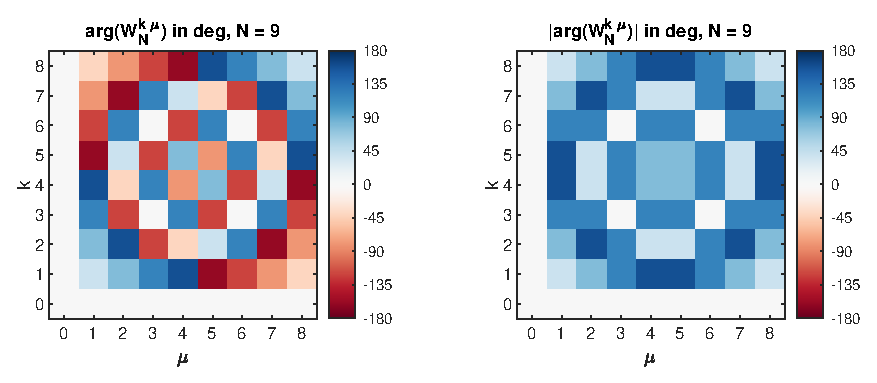
\includegraphics[]{graphics/TwiddleFactorMatrix_N9}
		\caption{$\text{arg}(W_N^{\mu k})$ (left) and $|\text{arg}(W_N^{\mu k}|$
		(right) as matrix over $\mu$ and $k$ for $N=9$.}
		\label{Twiddle2}
\end{figure}
\begin{figure}
		\centering
		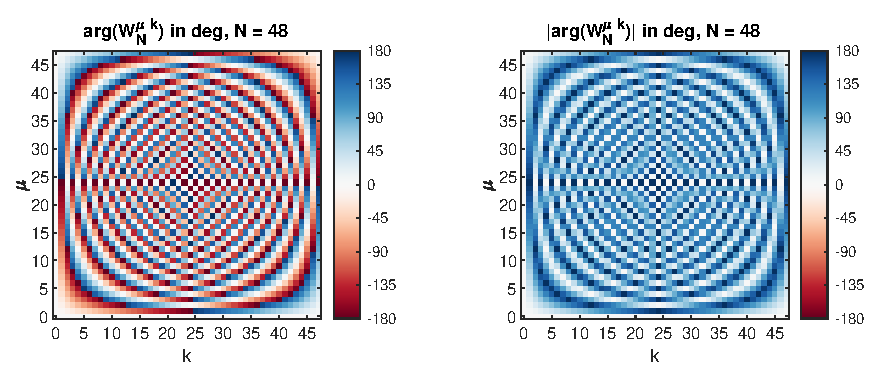
\includegraphics[]{graphics/TwiddleFactorMatrix_N48}
		\caption{$\text{arg}(W_N^{\mu k})$ (left) and $|\text{arg}(W_N^{\mu k})|$
		(right) as matrix over $\mu$ and $k$ for $N=48$.}
		\label{Twiddle3}
\end{figure}

% ---------------------------------------------------------------------------------
\subsection{DFT Frequency Resolution}
The relation between physical temporal frequency $f$, sampling frequency $f_s$
and discrete-time angular frequency $\Omega$ is known as
\begin{equation}
\Omega=2\pi \frac{f}{f_s}=\frac{\omega}{f_s}.
\end{equation}
%
Furthermore, the twiddle factor and the DFT matrix tell us that
the unit circle is equiangularly sampled, i.e. the angular frequency
resolution
\begin{equation}
\Delta \Omega = \frac{2\pi}{N}
\end{equation}
holds.
%
From both equations
\begin{equation}
\Delta \Omega=2\pi \frac{\Delta f}{f_s}=\frac{\Delta \omega}{f_s}\equiv
\Delta \Omega = \frac{2\pi}{N}
\end{equation}
we can deduce the DFT resolution in terms of the physical frequency $f$ as
\begin{equation}
\boxed{\Delta f = \frac{f_s}{N}}.
\end{equation}
%
This corresponds to the frequency distance between two spectral lines, i.e.
between two bins.
%
From that, all so called eigenfrequencies of the DFT, i.e. frequencies where
the DFT bins are located, can be derived as
\begin{equation}
\boxed{f_\text{DFT}=\mu \Delta f=\mu\frac{f_s}{N}
\hspace{5mm}\text{for}\hspace{5mm}
0\leq \mu\leq N-1,\,\,\mu\in\mathbb{N}}.
\end{equation}
%
These DFT eigenfrequencies can also be given for the discrete-time angular
frequency
\begin{equation}
\Omega_\text{DFT} =
\mu \Delta \Omega =
\mu \frac{2\pi}{N} =
\frac{2\pi f_\text{DFT}}{f_s}.
\label{eq:OmegaDFT}
\end{equation}

% -----------------------------------------------------------------------------
\subsection{Periodicity and Symmetry of the DFT}
The signals $x[k]$ and $X[\mu]$ of an DFT/IDFT pair exhibit a periodicity of $N$.
%
This is shown with $k,\mu,k',m\in\mathbb{Z}$:
\begin{align}
x[k']&=\frac{1}{N}\sum_{\mu=0}^{N-1}X[\mu]\e^{\im\frac{2\pi}{N}k'\mu}\\
x[k'=k+m N]&=\frac{1}{N}\sum_{\mu=0}^{N-1}X[\mu]\e^{\im\frac{2\pi}{N}(k+mN)\mu}\\
&=\frac{1}{N}\sum_{\mu=0}^{N-1}X[\mu]\e^{\im\frac{2\pi}{N}k\mu}\cdot\underbrace{\e^{\im\frac{2\pi}{N}mN\mu}}_{=1}=x[k].
\end{align}
%
A similar proof yields the identity $X[\mu]=X[\mu+mN]$, cf.
Fig.~\ref{Periodicity_DFT}.
%
This is equivalent to a DTFT spectrum that exhibits a $2\pi$ periodicity, i.e.
$X(\Omega)=X(\Omega+m\cdot2\pi)$.
%
The baseband of the DFT for $0\leq\mu\leq N-1$ corresponds to the spectrum of
the signal $x[k]$ for $0\leq k\leq N-1$.
%
Thus, both signals $x[k]$ and $X[\mu]$ inherently exhibit periodicity with $N$.
\begin{figure}
		\centering
		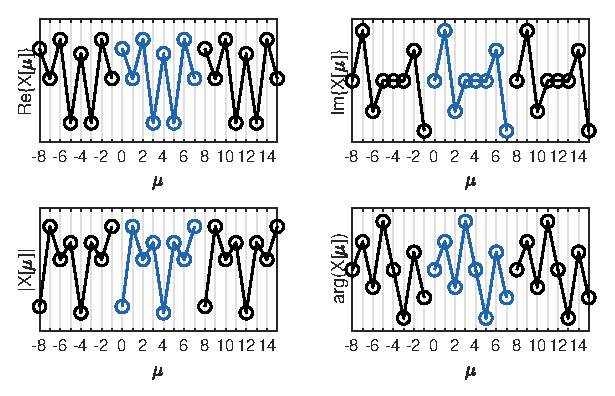
\includegraphics[width=12cm]{graphics/Periodicity_DFT}
		\caption{Periodicity of the DFT for a real signal with $N=8$,
		blue: baseband, black: periodic repetitions.}
		\label{Periodicity_DFT}
\end{figure}%

A further very important characteristic of the DFT spectrum is observed,
when $x[k]\in\mathbb{R}$ (such as audio and video signals) is assumed.
%
Then the symmetries
\begin{align}
\text{Re}\left\{X\left[\frac{N}{2}+m\right]\right\}&=\text{Re}\left\{X\left[\frac{N}{2}-m\right]\right\}, \hspace{5mm} \text{Im}\left\{X\left[\frac{N}{2}+m\right]\right\}=-\text{Im}\left\{X\left[\frac{N}{2}-m\right]\right\},\\
\left|X\left[\frac{N}{2}+m\right]\right|&=\left|X\left[\frac{N}{2}-m\right]\right|, \hspace{1.3cm} \arg\left(X\left[\frac{N}{2}+m\right]\right)=-\arg\left(X\left[\frac{N}{2}-m\right]\right)
\end{align}
%
hold that can be written shortly as
%
\begin{equation}
X\left[\frac{N}{2}+m\right]=X\left[\frac{N}{2}-m\right]^*,
\label{eq:Symmetry_DFT}
\end{equation}
%
with $()^*$ again denoting conjugate-complex operation.
%
Think of $N$ as being an even number here, so $m\in \mathbb{Z}$.
%
The case of odd-numbered $N$ is considered later.
%
The symmetry property of eq.~\eqref{eq:Symmetry_DFT} is shown by inserting and
simplifying
\begin{align}
X\left[\mu=\frac{N}{2}+m\right]&=\sum_{k=0}^{N-1}x[k]\e^{-\im\frac{2\pi}{N}k{\left(\frac{N}{2}+m\right)}}=\sum_{k=0}^{N-1}x[k]\e^{-\im\pi k}\cdot\e^{-\im\frac{2\pi}{N}km},\\
X\left[\mu=\frac{N}{2}-m\right]&=\sum_{k=0}^{N-1}x[k]\e^{-\im\frac{2\pi}{N}k{\left(\frac{N}{2}-m\right)}}=\sum_{k=0}^{N-1}x[k]\e^{-\im\pi k}\cdot\e^{\im\frac{2\pi}{N}km}.
\end{align}
%
The sum of two complex numbers $a,b\in\mathbb{C}$ is just $(a+b)^*=a^*+b^*$.
Recall that $\e^{-\im\pi k}=\pm 1\in\mathbb{R}$.
%
With the assumption $x[k]\in\mathbb{R}$ it can then be proved
\begin{align}
X\left[\mu=\frac{N}{2}-m\right]^*&=\left(\sum_{k=0}^{N-1}x[k]\e^{-\im\pi k}\cdot\e^{\im\frac{2\pi}{N}km}\right)^*\\
&=\sum_{k=0}^{N-1}x[k]\e^{-\im\pi k}\cdot\left(\e^{\im\frac{2\pi}{N}km}\right)^*\\
&=\sum_{k=0}^{N-1}x[k]\e^{-\im\pi k}\e^{-\im\frac{2\pi}{N}km}\\
&=X\left[\mu=\frac{N}{2}+m\right].
\end{align}
%
Since the discrete DFT spectrum is only defined at $\mu\in\mathbb{Z}$
$m$ must be defined as follows
\begin{align}
m=\begin{cases}M&\text{for even }N\\
M+\frac{1}{2}&\text{for odd }N\end{cases}
\end{align}
%
using $M\in\mathbb{Z}$, cf.~Fig.~\ref{Symmetry_DFT_N8} and Fig.~\ref{Symmetry_DFT_N9}.
%
\begin{figure}
		\centering
		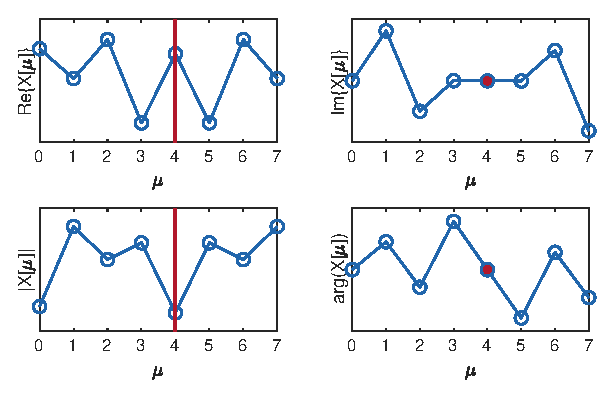
\includegraphics[]{graphics/Symmetry_DFT_N8}
		\caption{Symmetry of the DFT for $x[k]\in\mathbb{R}$ with $N=8$.
		Point and axis for symmetry is at $\frac{N}{2}=4$.
		Left: real part and magnitude of $X[\mu]$ are axisymmetric,
		right: imaginary part and phase of $X[\mu]$ are point-symmetric.}
		\label{Symmetry_DFT_N8}
\end{figure}
\begin{figure}
		\centering
		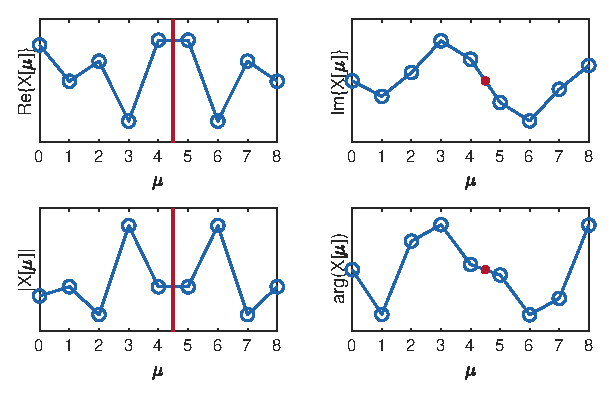
\includegraphics[]{graphics/Symmetry_DFT_N9}
		\caption{Symmetry of the DFT for $x[k]\in\mathbb{R}$ with $N=9$.
		Point and axis for symmetry is at $\frac{N}{2}=4.5$, i.e. between two DFT bins.
		Left: real part and magnitude of $X[\mu]$ are axisymmetric,
		right: imaginary part and phase of $X[\mu]$ are point-symmetric.}
		\label{Symmetry_DFT_N9}
\end{figure}
%
Due to the periodicity of $X[\mu]$ in general and the special $\frac{N}{2}$
symmetries of $X[\mu]$ when $x[k]\in\mathbb{R}$
(point-symmetric for imaginary part and phase, axisymmetric for real part and
magnitude, cf. again Fig.~\ref{Symmetry_DFT_N8} and Fig.~\ref{Symmetry_DFT_N9})
some information is redundant in the DFT spectrum.
%
For the interpretation of the DFT spectrum, only
\begin{align}
M&=\frac{N}{2}+1 \hspace{5mm}\text{for even }N\nonumber\\
M&=\frac{N+1}{2} \hspace{5mm}\text{for odd }N
\end{align}
bins contain non-redundant information.
%
This corresponds to the frequency band from DC ($f=0$ Hz) to half the sampling
frequency ($f_s/2$).
%
It is defined for \textbf{even} $N$ as
\begin{equation}
0\leq\mu\Delta f\leq\frac{f_s}{2} \hspace{5mm}\text{for}\hspace{5mm} 0\leq\mu\leq\frac{N}{2}
\end{equation}
and for \textbf{odd} $N$ as
\begin{equation}
0\leq\mu\Delta f<\frac{f_s}{2} \hspace{5mm}\text{for}\hspace{5mm} 0\leq\mu\leq\frac{N-1}{2}.
\end{equation}
%
Thus, for even $N$ the symmetry axis $\mu=\frac{N}{2}$ is exactly at the bin
indicating half of the sampling frequency
%
\begin{equation}
f=\mu\frac{f_s}{N}=\frac{N}{2}\frac{f_s}{N}=\frac{f_s}{2},
\end{equation}
%
whereas for odd $N$ the symmetry axis is located between the two bins around
$\frac{f_s}{2}$.
%
Therefore, an odd $N$ DFT does not include the 'half of the sampling frequency'
bin, cf.~Fig.~\ref{DFT_Eigenfrequenzen_N4_N5}, Fig.~\ref{DFT_Eigenfrequenzen_N8_N9}.

% -----------------------------------------------------------------------------
\subsection{DFT as Sampling of the DTFT}
The following discussion of the discrete Fourier transform (DFT) as a sampled
DTFT and explanations concerning windowing were inspired by the brilliant
script \cite{Moeser2011} and became extended. A very similar didactic concept
is approached in \cite[Ch.~7.3,~7.4]{Kammeyer2002}

The DFT contains all possible spectral information that can be derived from the
signal.
%
Since $N$ time samples are available, only maximum $N$ (complex valued) spectral
samples are available; for $x[k]\in\mathbb{R}$ less than $N$ samples contain
non-redundant information as shown above.
%
The DFT can be derived by sampling the DTFT spectrum equiangularly on the unit
circle with $\Delta\Omega=\frac{2\pi}{N}$,
cf.~Fig.~\ref{DFT_Eigenfrequenzen_N4_N5}, Fig.~\ref{DFT_Eigenfrequenzen_N8_N9}.
%
\begin{figure}
		\centering
		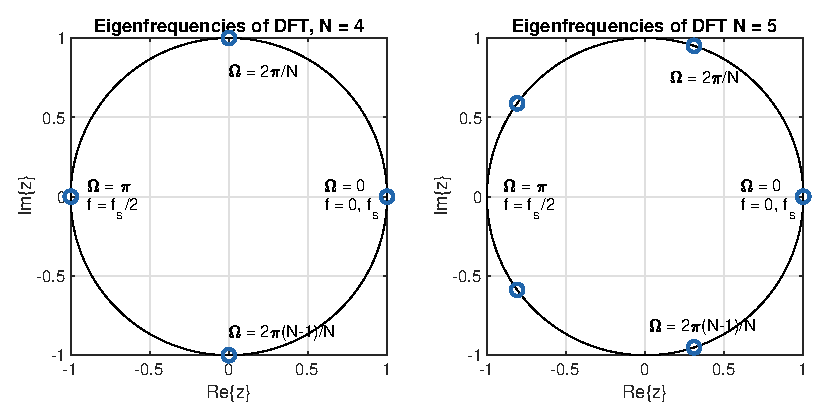
\includegraphics[]{graphics/DFT_Eigenfrequenzen_N4_N5}
		\caption{DFT eigenfrequency locations on the unit circle for $N=4$ (left),
		$N=5$ (right).}
		\label{DFT_Eigenfrequenzen_N4_N5}
\end{figure}
\begin{figure}
		\centering
		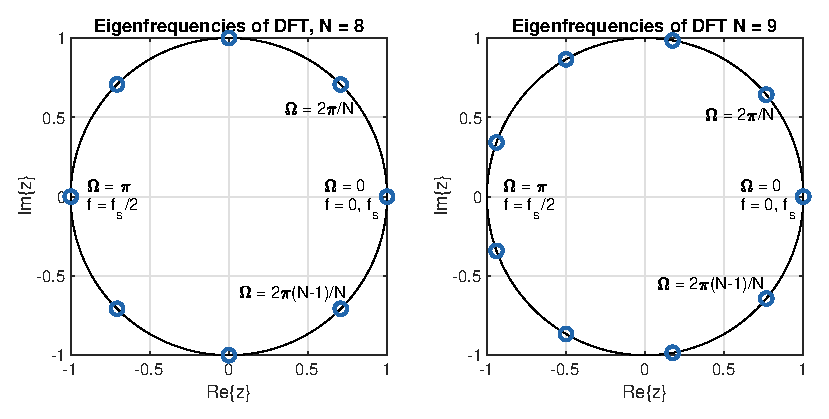
\includegraphics[]{graphics/DFT_Eigenfrequenzen_N8_N9}
		\caption{DFT eigenfrequency locations on the unit circle for $N=8$ (left),
		$N=9$ (right).}
		\label{DFT_Eigenfrequenzen_N8_N9}
\end{figure}
%
Thinking of the DFT $X[\mu]$ as being the spectrum of the non-zero part of a
sampled one-time signal $x[k]$ for $0\leq k\leq N-1$, $x[k]=0$ for all other
$k$ (so-called \textit{single signal model} \cite{Moeser2011}), inversely allows
for interpolation towards the DTFT spectrum.
%
To this end, the synthesis equation for the one-time signal eq.~\eqref{eq:IDFT}
%
\begin{equation}
x[k]=\frac{1}{N}\cdot\sum_{\mu=0}^{N-1}X[\mu]\cdot\e^{\im\frac{2\pi}{N}k\mu}
\end{equation}
%
is inserted into the analysis equation of the DTFT eq.~\eqref{eq:DTFT} and gets
rearranged:
\begin{align}
X(\Omega)&=\sum_{k=-\infty}^\infty x[k]\cdot\e^{-\im\Omega k}\\
&=\sum_{k=0}^{N-1}\frac{1}{N}\cdot\sum_{\mu=0}^{N-1}X[\mu]\cdot\e^{\im\frac{2\pi}{N}k\mu}\cdot\e^{-\im\Omega k}\\
&=\sum_{\mu=0}^{N-1}X[\mu]\cdot\frac{1}{N}\cdot\sum_{k=0}^{N-1}\e^{-\im k\left(\Omega-\frac{2\pi}{N}\mu\right)}.
\end{align}
%
The sum over $k$ is a geometric series and can be rearranged with
\cite[(3-39)]{Lyons2011} to
%
\begin{align}
X(\Omega)&=\sum_{\mu=0}^{N-1}X[\mu]\cdot\frac{1}{N}\cdot\frac{1-\e^{-\im\left(\Omega-\frac{2\pi}{N}\mu\right)N}}{1-\e^{-\im\left(\Omega-\frac{2\pi}{N}\mu\right)}}\\
&=\sum_{\mu=0}^{N-1}X[\mu]\cdot\frac{1}{N}\cdot\frac{\e^{-\im\frac{\left(\Omega-\frac{2\pi}{N}\mu\right)N}{2}}}{\e^{-\im\frac{\Omega-\frac{2\pi}{N}\mu}{2}}}\cdot\frac{\e^{\im\frac{\left(\Omega-\frac{2\pi}{N}\mu\right)N}{2}}-\e^{-\im\frac{\left(\Omega-\frac{2\pi}{N}\mu\right)N}{2}}}{\e^{\im\frac{\Omega-\frac{2\pi}{N}\mu}{2}}-\e^{-\im\frac{\Omega-\frac{2\pi}{N}\mu}{2}}}\\
&=\sum_{\mu=0}^{N-1}X[\mu]\cdot\frac{1}{N}\cdot\e^{-\im\frac{\left(\Omega-\frac{2\pi}{N}\mu\right)(N-1)}{2}}\cdot\frac{\e^{\im\frac{\left(\Omega-\frac{2\pi}{N}\mu\right)N}{2}}-\e^{-\im\frac{\left(\Omega-\frac{2\pi}{N}\mu\right)N}{2}}}{\e^{\im\frac{\Omega-\frac{2\pi}{N}\mu}{2}}-\e^{-\im\frac{\Omega-\frac{2\pi}{N}\mu}{2}}}.
\end{align}
%
With the Euler identity $2\im\cdot\sin(x)=\e^{\im x}-\e^{-\im x}$ this can be
simplified to \cite[eq.~(2.41)]{Moeser2011}
%
\begin{equation}
X(\Omega)=\sum_{\mu=0}^{N-1}X[\mu]\cdot\e^{-\im\frac{\left(\Omega-\frac{2\pi}{N}\mu\right)(N-1)}{2}}\cdot\frac{1}{N}\cdot\frac{\sin\left(N\frac{\Omega-\frac{2\pi}{N}\mu}{2}\right)}{\sin\left(\frac{\Omega-\frac{2\pi}{N}\mu}{2}\right)}.
\label{eq:DTFT_Interpolation}
\end{equation}
%
The interpolation kernel is the so-called aliased or periodic sinc function
%
\begin{align}
\text{psinc}_N(\Omega)=\begin{cases}\frac{1}{N}\cdot\frac{\sin\left(\frac{N}{2}\Omega\right)}{\sin\left(\frac{1}{2}\Omega\right)}&\text{for }\Omega\neq2\pi m\\
(-1)^{m(N-1)}&\text{for }\Omega=2\pi m\end{cases},\,\,m\in\mathbb{Z},
\label{eq:periodic_sinc}
\end{align}
%
in Matlab and Python's scipy \texttt{diric(Omega,N)}, and a phase shift.
%
Therefore, eq.~\eqref{eq:DTFT_Interpolation} can be written as
%
\begin{equation}
X(\Omega)=\sum_{\mu=0}^{N-1}X[\mu]\cdot\e^{-\im\frac{\left(\Omega-\frac{2\pi}{N}\mu\right)(N-1)}{2}}\cdot\text{psinc}_N\left(\Omega-\frac{2\pi}{N}\mu\right).
\label{eq:DTFT_Interpolation_psinc}
\end{equation}
%
Thus, a DTFT value at any $\Omega$ can be interpolated using
eq.~\eqref{eq:DTFT_Interpolation_psinc}.
%
It is easy to show, that for $\Omega=\frac{2\pi}{N}\mu'$ this evaluates exactly
to the DFT value since this is a DFT eigenfrequency:
\begin{align}
X\left(\Omega=\frac{2\pi}{N}\mu'\right)&=\sum_{\mu=0}^{N-1}X[\mu]\cdot\e^{-\im\frac{\left(\frac{2\pi}{N}\mu'-\frac{2\pi}{N}\mu\right)(N-1)}{2}}\cdot\frac{1}{N}\cdot\frac{\sin\left(N\frac{\frac{2\pi}{N}\mu'-\frac{2\pi}{N}\mu}{2}\right)}{\sin\left(\frac{\frac{2\pi}{N}\mu'-\frac{2\pi}{N}\mu}{2}\right)},\\
&=\sum_{\mu=0}^{N-1}X[\mu]\cdot\e^{-\im\frac{\pi(\mu'-\mu)(N-1)}{N}}\cdot\frac{1}{N}\cdot\frac{\sin(\pi(\mu'-\mu))}{\sin\left(\frac{\pi}{N}(\mu'-\mu)\right)}.
\end{align}
%
For all $\mu\neq\mu'$ the term $\sin(\pi(\mu'-\mu))=0$.
%
For $\mu=\mu'$ the periodic sinc evaluates to $1$ and
$e^{-\im\frac{\pi(\mu'-\mu)(N-1)}{N}}=1$.
%
Thus, the interpolation yields
\begin{equation}
X\left(\Omega=\frac{2\pi}{N}\mu'\right)=X[\mu'],
\end{equation}
and it can be seen that the DTFT and DFT spectrum are identical at all DFT
eigenfrequencies
%
\begin{equation}
\Omega_\text{DFT}=\frac{2\pi}{N}\mu \hspace{5mm}\text{for}\hspace{5mm} 0\leq\mu\leq N-1,\,\,\mu\in\mathbb{N}.
\end{equation}
%
For all other frequencies, the DTFT spectrum follows the interpolation kernel,
cf. Fig.~\ref{DTFT_Interpolation}.
%
\begin{figure}
		\centering
		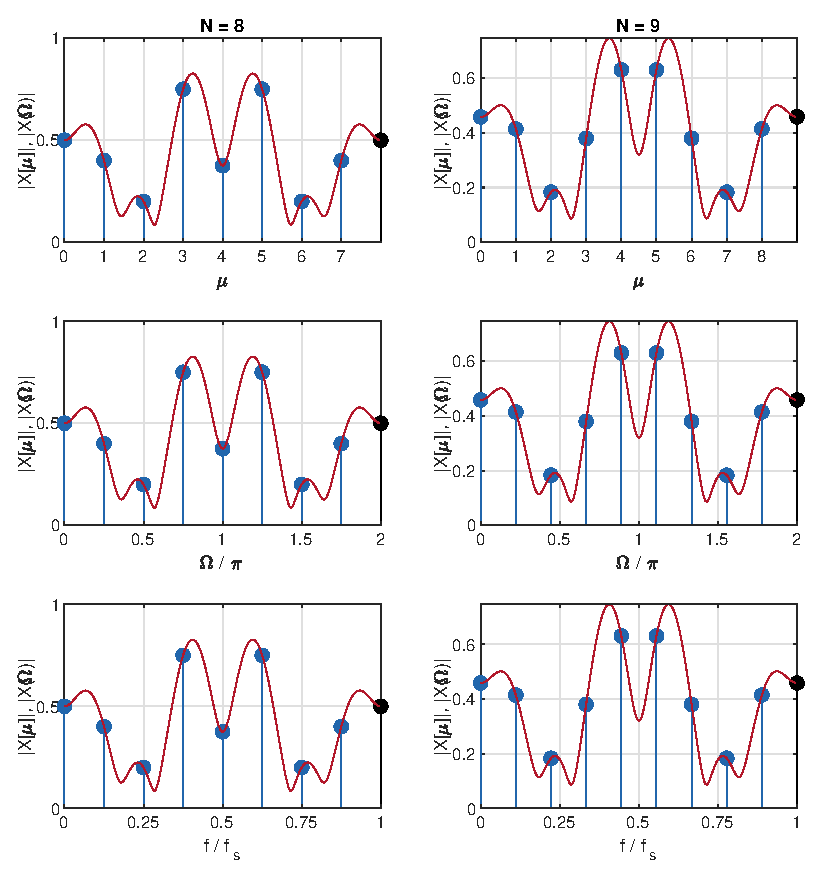
\includegraphics[]{graphics/DTFT_Interpolation}
		\caption{DFT (stem, blue) and interpolated DTFT (line, red) magnitude
		spectra over $\mu$ (top), $\Omega/\pi$ (middle) and $\frac{f}{f_s}$ (bottom)
		for $N=8$ (left) and $N=9$ (right).}
		\label{DTFT_Interpolation}
\end{figure}
%
As already introduced in eq.~\eqref{eq:OmegaDFT}
%
\begin{equation}
\Omega=\frac{2\pi f}{f_s} \hspace{1cm} \Omega_\text{DFT}=\frac{2\pi f_\text{DFT}}{f_s}
\end{equation}
hold as well.
%
Thus, a DFT and an interpolated DTFT spectrum can be visualised over $\mu$,
$\Omega$ and, for a given sampling frequency $f_s$, over $f$ as depicted in
Fig.~\ref{DTFT_Interpolation}.

% -----------------------------------------------------------------------------
\subsection{Windowing}
Many textbooks treat the derivation of the DFT and windowing separately, which
is sensible if the concept of the DFT is to be introduced solely as a transform.
%
For the spectral analysis of signals, it might be helpful to discuss the DFT
and windowing together as e.g. in \cite{Moeser2011},
\cite[Ch.~7.3,~7.4]{Kammeyer2002}.

Let $x[k]$ for $-\infty\leq k\leq\infty$ be a sequence with the corresponding
continuous and periodic DTFT spectrum $X(\Omega)$.
%
For a computer-assisted spectral analysis, it is necessary to cut out a finite
number of values out of a representative signal section.
%
Mathematically, this is described by multiplication with a weighting or window
sequence $w[k]$, that equals zero outside the desired signal section:
%
\begin{equation}
w[k]=0 \hspace{5mm} \text{for}\,\,k<0\,\,\text{and}\,\,k\geq N, \hspace{5mm} w\in\mathbb{R}.
\end{equation}
%
For example, the definition of a rectangular window is
%
\begin{equation}
w[k]=\left\{\begin{matrix}1 & \text{for} & 0\leq k\leq N-1\\0 & \text{otherwise} &\end{matrix}\right..
\end{equation}
%
Of course the chosen signal section does not have to start at $k=0$,
but it makes calculations easier.
%
The sequence $w[k]$ has a corresponding DTFT spectrum $W(\Omega)$ as well:
%
\begin{align}
W(\Omega)&=\sum_{k=-\infty}^{\infty}w[k]\e^{-\im\Omega k}\nonumber\\
w[k]&=\frac{1}{2\pi}\int\limits_{-\pi}^{\pi}W(\Omega)\e^{\im\Omega k}\text{d}\Omega.
\end{align}
%
Cutting-out the signal section means multiplication of the signal with the
window sequence
%
\begin{equation}
x_\text{N}[k]=x[k]\cdot w[k],
\end{equation}
%
which can be expressed as a cyclic convolution of the corresponding spectra in
the frequency domain:
%
\begin{align}
X_\text{N}(\Omega)&=\frac{1}{2\pi}(X\circledast W)(\Omega)\\
&=\frac{1}{2\pi}\int\limits_{-\pi}^{\pi}X(\Omega-\nu)\cdot W(\nu)\text{d}\nu\\
&= \frac{1}{2\pi}\int\limits_{-\pi}^{\pi}X(\nu)\cdot W(\Omega-\nu)\text{d}\nu.
\end{align}

The DTFT spectrum $X_\text{N}(\Omega)$ contains the "original" DTFT spectrum
$X(\Omega)$ that was to be analysed, but it is smeared due to the convolution
with the window spectrum.
%
The only possibility to obtain $X_\text{N}(\Omega)=X(\Omega)$ is to convolve
with a window that is the neutral element of the convolution
%
\begin{equation}
W_\delta(\Omega)=2\pi\sum_{n=-\infty}^{\infty}\delta(\Omega+2\pi n)
\end{equation}
%
which yields
%
\begin{equation}
X_\text{N}(\Omega)=\int\limits_{-\pi}^{\pi}X(\Omega-\nu)\cdot\delta(\nu)\text{d}\nu
=\int\limits_{-\pi}^{\pi}X(\nu)\cdot\delta(\Omega-\nu)\text{d}\nu=X(\Omega).
\end{equation}
%
However, $W_\delta(\Omega)$ corresponds to \cite[tab.~2.3, p.~90]{Oppenheim2010}
\begin{equation}
W_\delta(\Omega)=2\pi\sum\limits_{n=-\infty}^{\infty}\delta(\Omega+2\pi n) \hspace{5mm}\Laplace\hspace{5mm} w_\delta[k]=1 \hspace{5mm} \text{for}\,\,-\infty\leq k\leq\infty,
\end{equation}
which constitutes an infinitely long window.
%
For the time domain follows
\begin{equation}
x_\text{N}[k]=x[k]\cdot w_\delta[k]=x[k],
\end{equation}
which delivers a consistent theory, but is not helpful for practical computation.

Therefore, $w_\delta[k]$ is not a window that can be employed in practice
(and it is not actually not even a real "window" as it is constantly 1),
but it should be kept in mind that $W_\delta(\Omega)$ would be the ideal window
spectrum for the analysis of $x[k]$.
%
So one has to accept that instead of being able to analyse $x[k]$ and $X(\Omega)$,
only $x_N[k]$ and $X_\text{N}(\Omega)$ are available.
%
How well $X_\text{N}(\Omega)\approx X(\Omega)$ can be approximated is dependent
on the length $N$ of the cut out section, on the chosen section of $x[k]$ and
on the sequence $w[k]$ and its spectrum $W(\Omega)$, that are itself dependent
on $N$.

To illustrate the importance of the window spectrum, the signal spectrum of a
single harmonic oscillation with the angular frequency $0\leq\Omega_0<\pi$
is considered \cite[tab.~2.3, p.~90]{Oppenheim2010}
%
\begin{equation}
X_\delta(\Omega)=2\pi\sum_{n=-\infty}^{\infty}\delta(\Omega-\Omega_0+2\pi n).
\label{eq:DTFTspec_harmSchwingung}
\end{equation}
%
For $X_\text{N}(\Omega)$ follows from the convolution
$X_{\delta,\text{N}}(\Omega)=\frac{1}{2\pi}(X_\delta\circledast W)(\Omega)$
the spectrum of the window sequence shifted by $\Omega_0$
%
\begin{equation}
X_{\delta,\text{N}}(\Omega)=W(\Omega-\Omega_0).
\end{equation}
%
Therefore, one must be able to interpret the window spectrum to conclude on
$X_\text{N}(\Omega)$ or even $X(\Omega)$.
%
The next section starts discussion on the rectangular window which is the
`natural' window of the DFT definition as it just cuts out a section of the
signal where all values are weighted equally.

%------------------------------------------------------------------------------
\subsubsection{Rectangular Window}
A window $w[k]$ of length $N$ is defined with
%
\begin{equation}
w[k]=0 \hspace{5mm} \text{for}\,\,k<0\,\,\text{and}\,\,k\geq N,\hspace{5mm} w\in\mathbb{R}.
\end{equation}
%
For $0\leq k\leq N-1$, $w[k]$ can consist of arbitrary real numbers.
%
If $w[k]=1$ for this range, a so called rectangular window is obtained.
%
To determine the spectrum of a window, one can calculate the DTFT of the
infinite sequence $w[k]$, where only values of the sequence that are $\neq0$
have to be summed up:
%
\begin{equation}
W(\Omega)=\sum_{k=0}^{N-1}w[k]\cdot\e^{-\im\Omega k}.
\end{equation}
%
For the simple rectangular window this yields
%
\begin{equation}
W_\text{Rect}(\Omega)=\sum_{k=0}^{N-1}1\cdot\e^{-\im\Omega k}.
\label{eq:Ansatz_RectWin}
\end{equation}
%
This is a geometric series for which the closed form solution is known
\cite[(3-39)]{Lyons2011} as
%
\begin{equation}
W_\text{Rect}(\Omega)=\frac{1-\e^{-\im\Omega N}}{1-\e^{-\im\Omega}}.
\end{equation}
%
This expression can be rewritten as
%
\begin{equation}
W_\text{Rect}(\Omega)=\frac{\e^{-\im\frac{\Omega N}{2}}}{\e^{-\im\frac{\Omega}{2}}}\cdot\frac{\e^{\im\frac{\Omega N}{2}}-\e^{-\im\frac{\Omega N}{2}}}{\e^{\im\frac{\Omega}{2}}-\e^{-\im\frac{\Omega}{2}}}
=\e^{-\im\frac{\Omega(N-1)}{2}}\cdot\frac{\e^{\im\frac{\Omega N}{2}}-\e^{-\im\frac{\Omega N}{2}}}{\e^{\im\frac{\Omega}{2}}-\e^{-\im\frac{\Omega}{2}}}
\end{equation}
%
and with the Euler identity $2\im\cdot\sin(x)=\e^{\im x}-\e^{-\im x}$ be
simplified to (cf. \cite[(3-42)]{Lyons2011})
%
\begin{equation}
W_\mathrm{Rect}(\Omega)=\e^{-\im\frac{\Omega(N-1)}{2}}\cdot\frac{\sin\left(N\frac{\Omega}{2}\right)}{\sin\left(\frac{\Omega}{2}\right)}.
\label{eq:DTFT_RectWin}
\end{equation}
%
The spectrum $W_\text{Rect}(\Omega)$ is like all Fourier transformed sequences
$2\pi$-periodic.
%
For the following discussion, only the section of the base band
$-\pi\leq\Omega<\pi$ is considered.

For the magnitude spectrum only the fraction containing the sines has to be
evaluated because $\left|\e^{-\im\frac{\Omega(N-1)}{2}}\right|=1$.
%
With the rule of L'Hospital \cite[(1.4.15	)]{Nist2010} the rectangular
window at $\Omega=0$ is
%
\begin{equation}
W_\text{Rect}(\Omega=0)=N.
\end{equation}
%
This is the amplitude that is weighting the current mid frequency in the
convolution the strongest, the so-called maximum main lobe amplitude.
%
The zeros $W_\text{Rect}(\Omega)=0$ in the base band result with
$m\in\mathbb{Z}$, $m\neq0$ after considering the argument of the sine in the
numerator
%
\begin{equation}
N\frac{\Omega}{2}=m\pi,
\end{equation}
in
\begin{equation}
\Omega=\frac{2\pi}{N}m=\Delta\Omega\cdot m.
\end{equation}
%
The zeros are equidistantly spaced with $\Delta\Omega=\frac{2\pi}{N}$.
%
For odd $N$, $N-1$ zeros result for
\begin{equation}
m=\pm1,\,\pm2,\,\pm3,\,...\,\pm\frac{N-1}{2}.
\end{equation}
%
For even $N$, $N-1$ zeros result for
\begin{equation}
m=\pm1,\,\pm2,\,\pm3,\,...\,\pm\left(\frac{N}{2}-1\right),\,-\frac{N}{2}.
\end{equation}
%
In the last case, the last zero $m=-\frac{N}{2}$ is exactly at $\Omega=-\pi$.
%
As it is a $2\pi$-periodic spectrum this zero could be defined with
$m=\frac{N}{2}$ as $\Omega=\pi$, but this would be the same zero and it is not
counted twice.
%
For $m=0$, no zero can be found, but instead the main lobe, as has been
described above.

Fig.~\ref{RectWindow_DTFT_DFT_lin_asym} and \ref{RectWindow_DTFT_DFT_lin_sym}
illustrate the cases $N=4$ and $N=5$ for the DTFT of the rectangular window.
%
The $N-1$ zeros of the spectrum are clearly visible.
%
Fig.~\ref{RectWindow_DTFT_log_asym} and \ref{RectWindow_DTFT_log_sym} show the
spectra with a logarithmic amplitude.
%
Differing from the depiction here, textbooks mostly use normalised representations
of window spectra of the form $20\cdot\log_{10}W[\Omega=0]=0$~dB, that are
symmetric in $\Omega=0$, i.e. plotted over $-\pi\leq\Omega<\pi$.
%
\begin{figure}
		\centering
		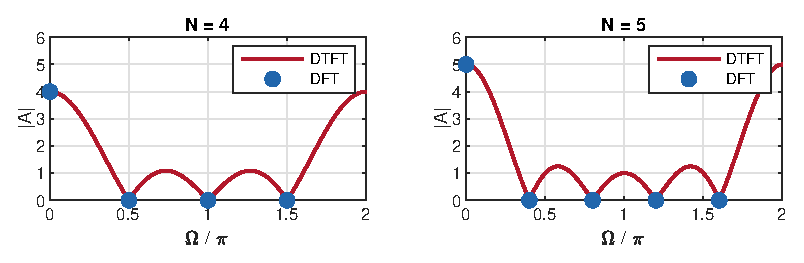
\includegraphics[]{graphics/RectWindow_DTFT_DFT_lin_asym}
		\caption{Magnitude of DTFT \& DFT spectra for rectangular windows of length
		$N$, $0\leq\Omega<2\pi$.}
		\label{RectWindow_DTFT_DFT_lin_asym}
\end{figure}
\begin{figure}
		\centering
		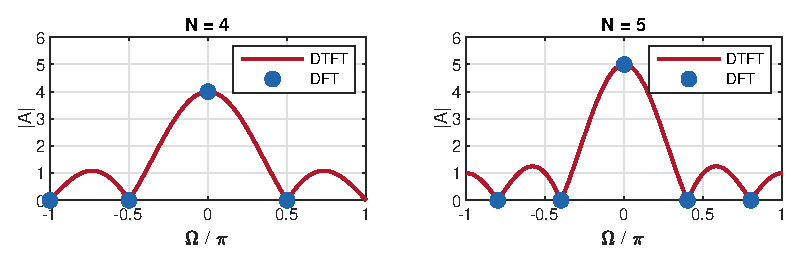
\includegraphics[]{graphics/RectWindow_DTFT_DFT_lin_sym}
		\caption{Magnitude of DTFT \& DFT spectra for rectangular windows of length
		$N$, $-\pi\leq\Omega<\pi$.}
		\label{RectWindow_DTFT_DFT_lin_sym}
\end{figure}
\begin{figure}
		\centering
		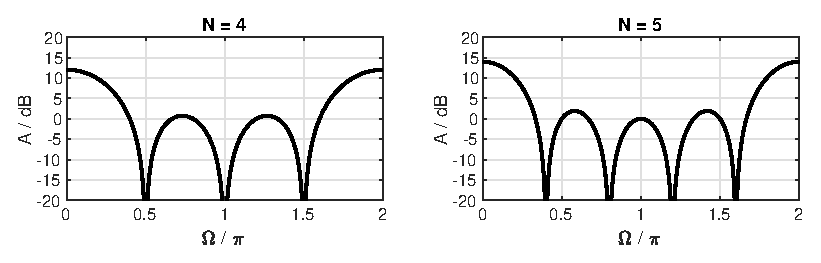
\includegraphics[]{graphics/RectWindow_DTFT_log_asym}
		\caption{Level of DTFT spectra for rectangular windows of length $N$,
		$0\leq\Omega<2\pi$.}
		\label{RectWindow_DTFT_log_asym}
\end{figure}
\begin{figure}
		\centering
		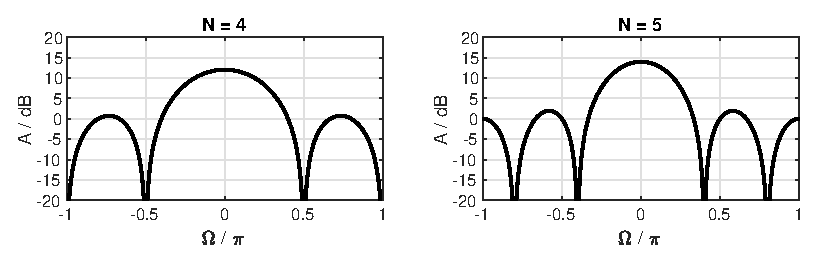
\includegraphics[]{graphics/RectWindow_DTFT_log_sym}
		\caption{Level of DTFT spectra for rectangular windows of length $N$,
		$-\pi\leq\Omega<\pi$.}
		\label{RectWindow_DTFT_log_sym}
\end{figure}

%------------------------------------------------------------------------------
\subsubsection{Discrete Spectrum of the Rectangular Window}
As has been explained before, the spectrum from eq.~\eqref{eq:DTFTspec_harmSchwingung}
%
\begin{equation}
X_\delta(\Omega)=2\pi\sum\limits_{n=-\infty}^\infty\delta(\Omega-\Omega_0+2\pi n)
\end{equation}
%
evolves with windowing, i.e. the convolution
$X_{\delta,\text{N}}(\Omega)=\frac{1}{2\pi}\,(X_\delta\circledast W)(\Omega)$,
into
%
\begin{equation}
X_{\delta,\text{N}}(\Omega)=W(\Omega-\Omega_0).
\end{equation}
%
Now, the spectrum of a finite signal is considered, i.e. a transition from the
DTFT to the DFT is performed.
%
For the discrete DFT frequencies that contain the complete spectral information,
$X_\delta[\mu]$ can be written as
%
\begin{equation}
X_\delta[\mu]=W\left[\frac{2\pi}{N}\mu-\Omega_0\right].
\end{equation}
%
With eq.~\eqref{eq:DTFT_RectWin} follows
%
\begin{align}
X_\delta[\mu]=W_\text{Rect}\left[\frac{2\pi}{N}\mu-\Omega_0\right]&=\e^{-\im\frac{\left(\frac{2\pi}{N}\mu-\Omega_0\right)(N-1)}{2}}\cdot\frac{\sin\left(N\frac{\frac{2\pi}{N}\mu-\Omega_0}{2}\right)}{\sin\left(\frac{\frac{2\pi}{N}\mu-\Omega_0}{2}\right)}\\
&=\e^{-\im\left(\frac{N-1}{2}\left(\frac{2\pi}{N}\mu-\Omega_0\right)\right)}\cdot\frac{\sin\left(\frac{N}{2}\left(\frac{2\pi}{N}\mu-\Omega_0\right)\right)}{\sin\left(\frac{1}{2}\left(\frac{2\pi}{N}\mu-\Omega_0\right)\right)}.
\label{eq:DFTspec_RectWin}
\end{align}
%
As can be seen, the DFT coefficients $X_\delta[\mu]$ strongly depend on
the choice of $\Omega_0$, which will be illustrated in the following.
%
The definition
%
\begin{equation}
\Omega_0=\frac{2\pi}{N}(\mu_0+\alpha)
\hspace{5mm} \text{with} \hspace{5mm}
\pm\alpha\leq\frac{1}{2}
\end{equation}
%
is inserted into eq.~\eqref{eq:DFTspec_RectWin} to yield
%
\begin{align}
X_\delta[\mu]&=\e^{-\im\left(\frac{N-1}{2}\left(\frac{2\pi}{N}\mu-\frac{2\pi}{N}(\mu_0+\alpha)\right)\right)}\cdot\frac{\sin\left(\frac{N}{2}\left(\frac{2\pi}{N}\mu-\frac{2\pi}{N}(\mu_0+\alpha)\right)\right)}{\sin\left(\frac{1}{2}\left(\frac{2\pi}{N}\mu-\frac{2\pi}{N}(\mu_0+\alpha)\right)\right)}\\
&=\e^{-\im\left(\frac{N-1}{2}\left(\frac{2\pi}{N}(\mu-\mu_0)-\frac{2\pi}{N}\alpha\right)\right)}\cdot\frac{\sin\left(\pi((\mu-\mu_0)-\alpha)\right)}{\sin\left(\frac{\pi}{N}((\mu-\mu_0)-\alpha)\right)}.
\label{eq:DFTspec_mitalpha}
\end{align}
%
For the case $\alpha=0$, we have $\Omega_0=\frac{2\pi}{N}\mu_0$ and the fraction
containing the sines evaluates to $N$ (cf. periodic sinc in
eq.~\eqref{eq:periodic_sinc}), so the DFT spectrum becomes
%
\begin{equation}
X_\delta[\mu]=\left\{\begin{matrix}0 & \text{for} & \mu\neq\mu_0\\N & \text{for} & \mu=\mu_0\end{matrix}\right..
\end{equation}
%
Therefore, if the chosen frequency from eq.~\eqref{eq:DTFTspec_harmSchwingung}
happens to be a DFT bin, the frequency spectrum contains the exact amplitude of
this frequency (after normalising with $\frac{1}{N}$).
%
The other values of the spectrum coincide with the zeros of the window spectrum.
%
This is the best case because the amplitude of the frequency $\Omega_0$ can be
analysed exactly, cf. Fig.~\ref{DFTbestworstcase_RectWin} left.
%
The worst case occurs when $\alpha=\pm\frac{1}{2}$.
%
For the rectangular window, two bins share the main energy and the other bins
differ from zero as well, cf. Fig.~\ref{DFTbestworstcase_RectWin} right.
%
It is not as easy anymore how to interpret the DFT spectrum.
%
From the example it is known that the signal consists of only one spectral
component, but in the spectrum this is not so obvious.
%
So what is to do when the frequencies and corresponding amplitudes of the signal
are not known (as is of course usually the case in real applications)?
%
\begin{figure}
		\centering
		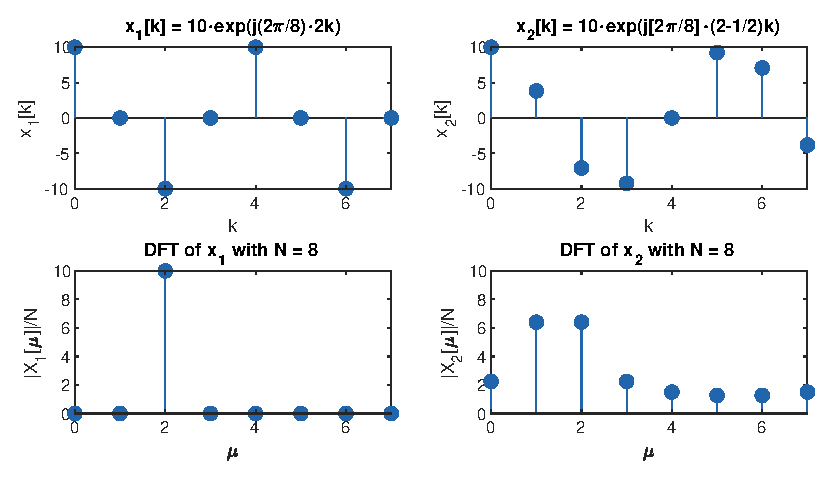
\includegraphics[]{graphics/DFTbestworstcase_RectWin}
		\caption{Rectangular windowing for $N=8$,
		best case ($\mu=2$), worst case ($\mu=2-\frac{1}{2}$).}
		\label{DFTbestworstcase_RectWin}
\end{figure}

For the interpretation of such spectra, knowledge about windowing and different
window types as well as experience in analysing spectra is necessary.
%
In a first step one can determine for each window which amplitude error arises
between best and worst case.
%
This gives an indication for the "true" spectrum.
%
For the rectangular window, this calculation is quite easy and is shown here:
%
With eq.~\eqref{eq:DFTspec_mitalpha}, the amplitude for a certain $\mu_0$ is
generally
%
\begin{equation}
|X_\delta[\mu_0]|=\left|\frac{\sin(-\pi\alpha)}{\sin\left(-\frac{\pi}{N}\alpha\right)}\right|
=\left|\frac{\sin(\pi\alpha)}{\sin\left(\frac{\pi}{N}\alpha\right)}\right|
\end{equation}
%
and for the worst case $\alpha=\pm\frac{1}{2}$
%
\begin{equation}
|X_\delta[\mu_0]|=\left|\frac{\sin\left(\pm\frac{\pi}{2}\right)}{\sin\left(\pm\frac{\pi}{2N}\right)}\right|
=\left|\frac{\pm1}{\pm\sin\left(\frac{\pi}{2N}\right)}\right|
=\left|\frac{1}{\sin\left(\frac{\pi}{2N}\right)}\right|.
\end{equation}
%
For very large $N$, this yields due to $\sin(x)\approx x$ for small $x$ the
amplitude
%
\begin{equation}
|X_\delta[\mu_0]|=\frac{2N}{\pi}.
\end{equation}
%
The amplitude error between the best case for $\alpha=0$ and the worst case for
$\alpha=\pm\frac{1}{2}$ is then for large $N$
%
\begin{equation}
\frac{\left|X_\delta[\mu_0]_{\alpha=\pm\frac{1}{2}}\right|}{\left|X_\delta[\mu_0]_{\alpha=0}\right|}\approx\frac{\frac{2N}{\pi}}{N}\approx\frac{2}{\pi}\approx0.6366\,\hat{=}\,-3.9224\,\text{dB}.
\end{equation}
%
The amplitude loss from the value 10 to approx. 6.3 can be found in
Fig.~\ref{DFTbestworstcase_RectWin}.
%
It is still not known, though, which frequencies the signal consists of
($\mu=1$ or $\mu=2$ or both?).
%
This could be accomplished by an increase of $N$.
%
Additionally, the quite high amplitudes in the other bins are confusing.
%
This point can be counteracted with a window with a higher side lobe
attenuation that is presented in the next subsection discussing the Hanning
window.

%------------------------------------------------------------------------------
\subsubsection{Hanning Window}
\begin{figure}
		\centering
		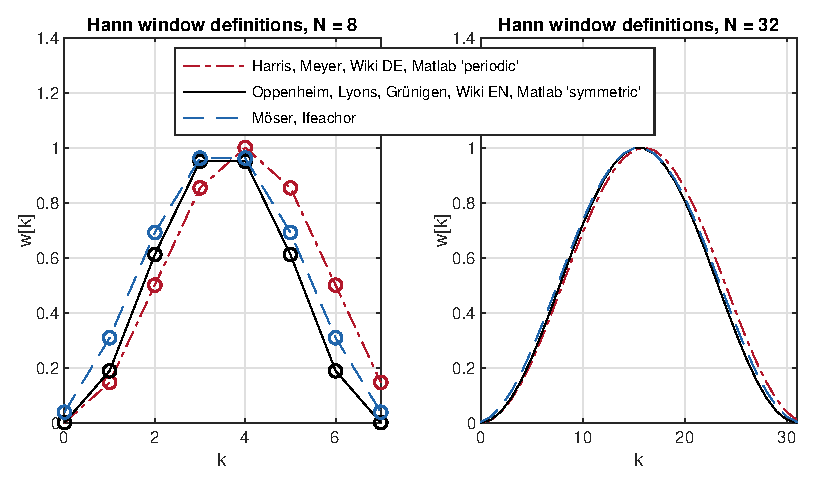
\includegraphics[]{graphics/HannDefinitionen}
		\caption{Different definitions of the Hanning window.}
		\label{HannDefinitionen}
\end{figure}

For the Hanning window (and for other windows as well), different definitions
exist in the literature.
%
Fig.~\ref{HannDefinitionen} shows differently defined Hanning windows for two
lengths $N$.
%
The red line starts at $w[k=0]=0$, but ends with $w[k=N-1]\neq0$.
%
This is based upon the reason that (at least for spectral analysis) a symmetric
window is not necessary \cite[p.~52]{Harris1978}.
%
Instead, the window is constructed in a such a way that for periodic extension
$w[N]=w[0]$.
%
The black line defines a window that is symmetric around $\frac{N-1}{2}$ and at
both terminal points $w[k=0]=0$ and $w[k=N-1]=0$ holds, because of the common
reasoning that the windowed signal must be zero at the terminal points to
ensure continuous transitions for periodic repetitions
\cite{Oppenheim2010, Lyons2011}.
%
The blue curve defines a window that is symmetric around $\frac{N-1}{2}$ as well,
but both terminal points $w[k=0]\neq0$ and $w[k=N-1]\neq0$.
%
The reason for this is that $N$ `real' DFT bins should be retrieved
\cite{Moeser2011, Ifeachor2002}.
%
This is why the sequence $w[k]$ for the blue line consists of $N$ coefficients
that differ from 0 while it is only $N-2$ for the black line.
%
A DFT of length $N$ for a sequence with only $N-2$ coefficients differing from
0 yields only $N-2$ `real' bins (compare to zero-padding).
%
For scientific purposes, it should be stated which definition of a standard
window has been used.

The application can determine which definition of a window is appropriate.
%
For spectral analysis a window should be used that can be extended periodically
without losing information in bins.
%
Those windows do not have to be symmetric around the middle of the window.
%
In FIR filter design one aims at reducing an infinite impulse response to a
finite length.
%
This is mostly done by symmetric windows to window symmetrically around the main
peak of the impulse response.
%
Therefore, Matlab discriminates between the variants \texttt{periodic} and
\texttt{symmetric} in window design.

Here, the window definition of \cite{Moeser2011} is used, although the Matlab
window as \texttt{periodic} version would be better suited, but the calculation
is easier.
%
For the window $w[k]$ of length $N$,
%
\begin{equation}
w[k]=0 \hspace{5mm} \text{for}\,\,k<0\,\,\text{and}\,\,k\geq N,
\hspace{5mm} w\in\mathbb{R}
\end{equation}
%
is still valid.
%
For $0\leq k\leq N-1$, $w[k]$ shall consist of arbitrary real numbers.
%
In this case here, those numbers are the ones of a Hanning window.
%
Additionally, the window should be symmetric
%
\begin{equation}
w[N-1-k]=w[k]
\end{equation}
%
and without zeros in the definition range.
%
The Hanning window version that fulfills this reads
%
\begin{align}
w[k]=\left\{\begin{matrix}1-\cos\left(\frac{2\pi}{N}\left(k+\frac{1}{2}\right)\right) & \text{for} & 0\leq k\leq N-1\\0 & \text{else} & \end{matrix}\right..
\label{eq:hanning}
\end{align}
%
The spectrum can be calculated with the help of
\begin{equation}
\cos\left(\frac{2\pi}{N}\left(k+\frac{1}{2}\right)\right)=\frac{1}{2}\left(\e^{\im\frac{\pi}{N}}\e^{\im\frac{2\pi}{N}k}+\e^{-\im\frac{\pi}{N}}\e^{-\im\frac{2\pi}{N}k}\right)
\end{equation}
%
and
%
\begin{equation}
W(\Omega)=\sum\limits_{k=0}^{N-1}w[k]\e^{-\im\Omega k}.
\end{equation}
%
Therefore, the spectrum of the window is
%
\begin{align}
W_{\text{Hann}}(\Omega)&=\sum\limits_{k=0}^{N-1}\left(1-\cos\left(\frac{2\pi}{N}\left(k+\frac{1}{2}\right)\right)\right)\e^{-\im\Omega k}\\
&=\sum\limits_{k=0}^{N-1}\left(1-\frac{1}{2}\left(\e^{\im\frac{\pi}{N}}\e^{\im\frac{2\pi}{N}k}+\e^{-\im\frac{\pi}{N}}\e^{-\im\frac{2\pi}{N}k}\right)\right)\e^{-\im\Omega k}\\
&=\sum\limits_{k=0}^{N-1}\e^{-\im\Omega k}-\frac{1}{2}\e^{\im\frac{\pi}{N}}\sum\limits_{k=0}^{N-1}\e^{-\im\left(\Omega-\frac{2\pi}{N}\right)k}-\frac{1}{2}\e^{-\im\frac{\pi}{N}}\sum\limits_{k=0}^{N-1}\e^{-\im\left(\Omega+\frac{2\pi}{N}\right)k}.
\end{align}
%
Using the results for the rectangular windows
(cf. eq.~\eqref{eq:Ansatz_RectWin}), this can be abbreviated to
%
\begin{equation}
W_{\text{Hann}}(\Omega)=W_{\text{Rect}}(\Omega)-\frac{1}{2}\e^{\im\frac{\pi}{N}}W_{\text{Rect}}(\Omega-\frac{2\pi}{N})-\frac{1}{2}\e^{-\im\frac{\pi}{N}}W_{\text{Rect}}(\Omega+\frac{2\pi}{N}).
\end{equation}
%
As can be seen, the spectrum of the Hanning window is composed of the spectrum
of a rectangular window and two weighted spectra of rectangular windows
that are shifted by one bin.
%
With eq.~\eqref{eq:DTFT_RectWin}, this can be rewritten as
%
\begin{align}
W_{\text{Hann}}(\Omega)=&\e^{-\im\frac{\Omega(N-1)}{2}}\cdot\frac{\sin\left(N\frac{\Omega}{2}\right)}{\sin\left(\frac{\Omega}{2}\right)}\nonumber\\
&-\frac{1}{2}\e^{\im\frac{\pi}{N}}\e^{-\im\frac{(\Omega-\frac{2\pi}{N})(N-1)}{2}}\cdot\frac{\sin\left(N\frac{\Omega-\frac{2\pi}{N}}{2}\right)}{\sin\left(\frac{\Omega-\frac{2\pi}{N}}{2}\right)}\nonumber\\
&-\frac{1}{2}\e^{-\im\frac{\pi}{N}}\e^{-\im\frac{(\Omega+\frac{2\pi}{N})(N-1)}{2}}\cdot\frac{\sin\left(N\frac{\Omega+\frac{2\pi}{N}}{2}\right)}{\sin\left(\frac{\Omega+\frac{2\pi}{N}}{2}\right)}\\
=&\e^{-\im\frac{\Omega(N-1)}{2}}\cdot\frac{\sin\left(\frac{N}{2}\Omega\right)}{\sin\left(\frac{1}{2}\Omega\right)}\nonumber\\
&-\frac{1}{2}\e^{\im\frac{\pi}{N}}\e^{-\im\frac{(\Omega-\frac{2\pi}{N})(N-1)}{2}}\cdot\frac{\sin\left(\frac{N}{2}\left(\Omega-\frac{2\pi}{N}\right)\right)}{\sin\left(\frac{1}{2}\left(\Omega-\frac{2\pi}{N}\right)\right)}\nonumber\\
&-\frac{1}{2}\e^{-\im\frac{\pi}{N}}\e^{-\im\frac{(\Omega+\frac{2\pi}{N})(N-1)}{2}}\cdot\frac{\sin\left(\frac{N}{2}\left(\Omega+\frac{2\pi}{N}\right)\right)}{\sin\left(\frac{1}{2}\left(\Omega+\frac{2\pi}{N}\right)\right)}.
\end{align}
%
Because
%
\begin{equation}
\e^{\im\frac{\pi}{N}}\e^{-\im\frac{(\Omega-\frac{2\pi}{N})(N-1)}{2}}=\e^{-\im\frac{\Omega(N-1)}{2}}\e^{\im\frac{\pi}{N}}\e^{\im\frac{(N-1)}{2}\frac{2\pi}{N}}
=\e^{-\im\frac{\Omega(N-1)}{2}}\underbrace{\e^{\im\pi\left(\frac{1}{N}+\frac{N-1}{N}\right)}}_{=-1}
\end{equation}
%
and
%
\begin{equation}
\e^{-\im\frac{\pi}{N}}\e^{-\im\frac{(\Omega+\frac{2\pi}{N})(N-1)}{2}}=\e^{-\im\frac{\Omega(N-1)}{2}}\e^{-\im\frac{\pi}{N}}\e^{-\im\frac{(N-1)}{2}\frac{2\pi}{N}}
=\e^{-\im\frac{\Omega(N-1)}{2}}\underbrace{\e^{-\im\pi\left(\frac{1}{N}+\frac{N-1}{N}\right)}}_{=-1},
\end{equation}
%
the spectrum can be simplified to
%
\begin{align}
W_{\text{Hann}}(\Omega)&=\e^{-\im\frac{\Omega(N-1)}{2}}\cdot\frac{\sin\left(\frac{N}{2}\Omega\right)}{\sin\left(\frac{1}{2}\Omega\right)}+\frac{1}{2}\e^{-\im\frac{\Omega(N-1)}{2}}\cdot\frac{\sin\left(\frac{N}{2}\left(\Omega-\frac{2\pi}{N}\right)\right)}{\sin\left(\frac{1}{2}\left(\Omega-\frac{2\pi}{N}\right)\right)}+\frac{1}{2}\e^{-\im\frac{\Omega(N-1)}{2}}\cdot\frac{\sin\left(\frac{N}{2}\left(\Omega+\frac{2\pi}{N}\right)\right)}{\sin\left(\frac{1}{2}\left(\Omega+\frac{2\pi}{N}\right)\right)}\\
&=\e^{-\im\frac{\Omega(N-1)}{2}}\cdot\left(\frac{\sin\left(\frac{N}{2}\Omega\right)}{\sin\left(\frac{1}{2}\Omega\right)}+\frac{1}{2}\cdot\frac{\sin\left(\frac{N}{2}\left(\Omega-\frac{2\pi}{N}\right)\right)}{\sin\left(\frac{1}{2}\left(\Omega-\frac{2\pi}{N}\right)\right)}+\frac{1}{2}\cdot\frac{\sin\left(\frac{N}{2}\left(\Omega+\frac{2\pi}{N}\right)\right)}{\sin\left(\frac{1}{2}\left(\Omega+\frac{2\pi}{N}\right)\right)}\right).
\end{align}

The Hanning window exhibits only $N-3$ zeros compared to the rectangular window
with $N-1$ zeros, so two zeros are lost for usage in spectral shaping,
cf. fig~\ref{HanningausRectWindow} and \ref{DTFTHanningWin_lin}.
%
In the region close to $\Omega=\pm\pi$, the weighted and shifted spectra of
the rectangular windows (red and dark blue line) cancel out, which can be
observed in the logarithmic depiction in Fig.~\ref{DTFTHanningWin_log} as well,
i.e. the Hanning window achieves a better side lobe attenuation than the
rectangular window.
%
Around $\Omega\approx 0$, all three spectral components add up in a constructive
way, which leads to a broader main lobe compared to the rectangular window.
%It is worth to realize that no window can have a narrower main lobe than the rect
%window.

\begin{figure}
		\centering
		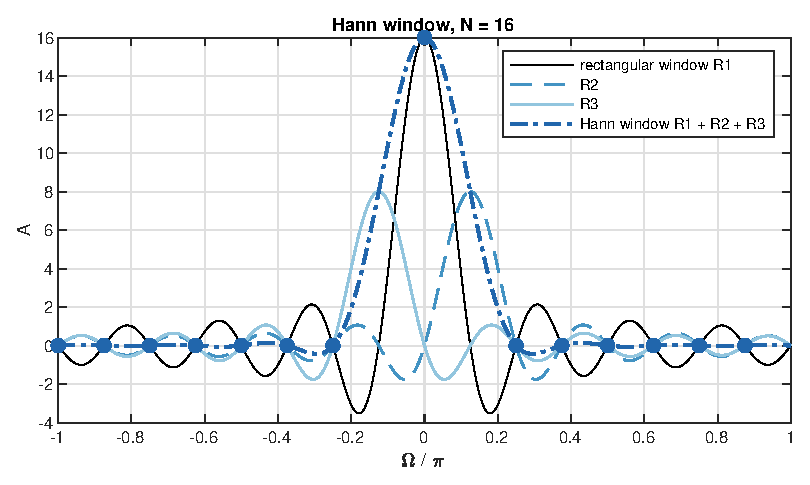
\includegraphics[]{graphics/HanningausRectWindow}
		\caption{Spectrum of Hanning window from superposition of weighted rectangular windows.}
		\label{HanningausRectWindow}
\end{figure}
\begin{figure}
		\centering
		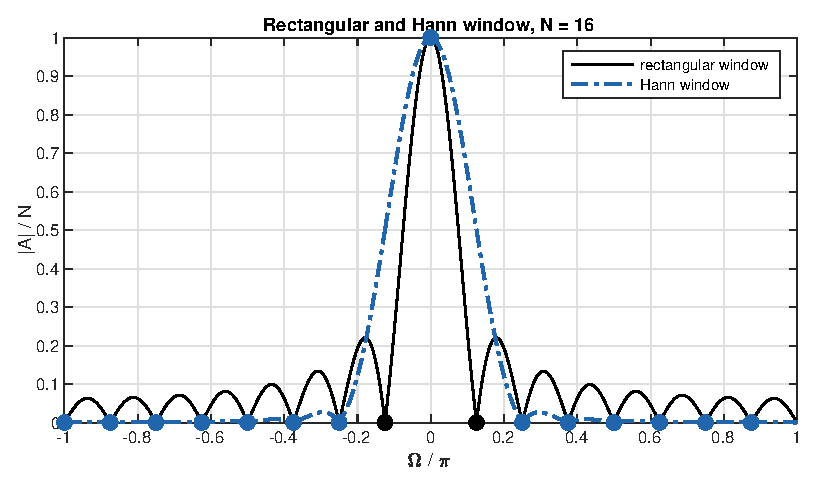
\includegraphics[]{graphics/DTFTHanningWin_lin}
		\caption{Magnitude of DTFT spectra for rectangular and Hanning window, $-\pi\leq\Omega<\pi$.}
		\label{DTFTHanningWin_lin}
\end{figure}
\begin{figure}
		\centering
		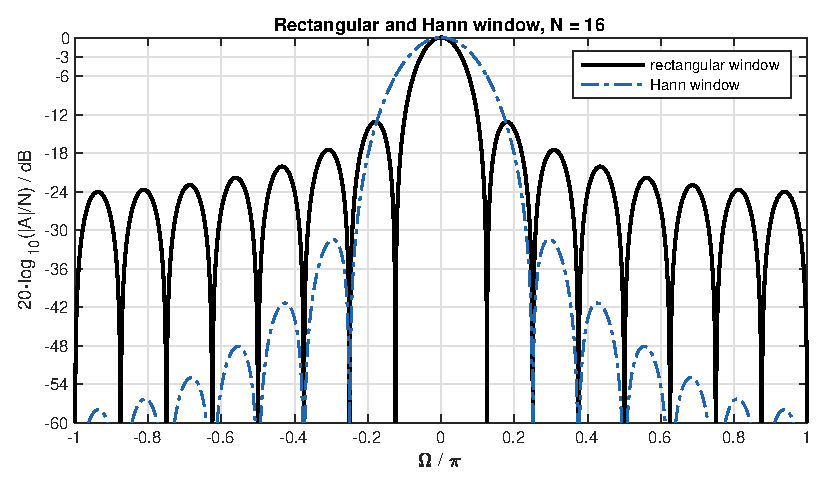
\includegraphics[]{graphics/DTFTHanningWin_log}
		\caption{Level of DTFT spectra for rectangular and Hanning window, $-\pi\leq\Omega<\pi$.}
		\label{DTFTHanningWin_log}
\end{figure}
\begin{figure}
		\centering
		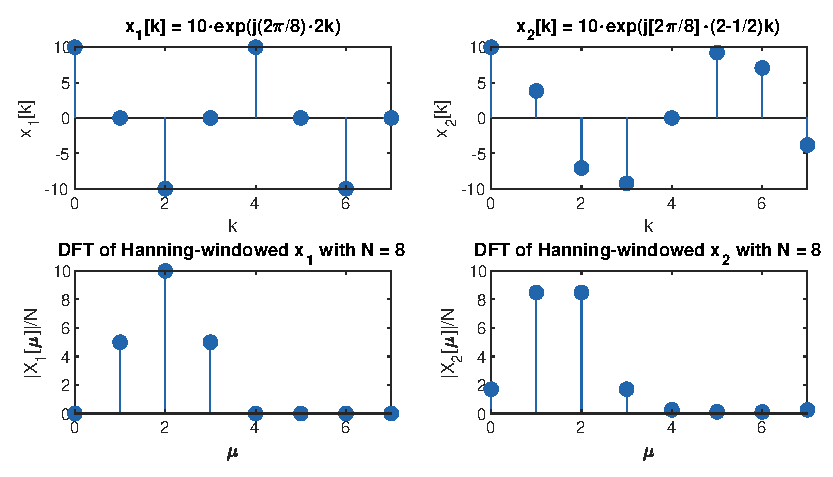
\includegraphics[]{graphics/DFTbestworstcase_HannWin}
		\caption{Hanning windowing for $N=8$, best case ($\mu=2$), worst case ($\mu=2-\frac{1}{2}$).}
		\label{DFTbestworstcase_HannWin}
\end{figure}

Fig.~\ref{DFTbestworstcase_HannWin} illustrates the best and worst case
scenarios for the Hanning window when a discrete frequency exactly coincides
with a DFT bin (left, best) or lies in the middle between two bins (right, worst).
%
In contrast to the rectangular window, the exact case ($\mu=2$, left) leads to
three bins that are differing from zero with the middle bin representing the
exact amplitude of the discrete frequency.
%
The worst case ($\mu=2-\frac{1}{2}$, right) leads to two main bins and further
bins differing from zero.
%
The amplitude error between best and worst case for large $N$ is
%
\begin{equation}
\frac{\left|X[\mu_0]_{\alpha=\pm\frac{1}{2}}\right|}{\left|X[\mu_0]_{\alpha=0}\right|}=\frac{3\pi}{8}\approx1.1781\,\hat{=}\,-1.4236\,\text{dB},
\end{equation}
%
which is smaller than the error for the rectangular window.
%
This discloses the following rule: The broader the main lobe of a window,
the smaller the amplitude error in spectal analysis for a harmonic signal with
the frequency
%
\begin{equation}
\Omega_0=\frac{2\pi}{N}(\mu_0+\alpha) \hspace{5mm} \text{with} \hspace{5mm} \pm\alpha\leq\frac{1}{2}.
\end{equation}
%
However, a broad main lobe leads to a poor frequency resolution, i.e.
frequencies that are close together get smeared in the convolution process
$X_N(\Omega)=\frac{1}{2\pi}(X_N\circledast W)(\Omega)$ and cannot be separated
clearly anymore. So, there is always a compromise involved in frequency
resolution and amplitude resolution.

One last remark on the amplitudes of the windows: In the literature, windows
are often normalised to a maximum value $=1$, which reads for
the Hanning window according to \cite{Moeser2011}
%
\begin{align}
w[k]=\left\{\begin{matrix}0.5-0.5\cos\left(\frac{2\pi}{N}\left(k+\frac{1}{2}\right)\right) & \text{for} & 0\leq k\leq N-1\\0 & \text{else} &\end{matrix}\right..
\end{align}
%
The definition that has been used above (cf. eq.~\eqref{eq:hanning}),
\begin{align}
w[k]=\left\{\begin{matrix}1-\cos\left(\frac{2\pi}{N}\left(k+\frac{1}{2}\right)\right) & \text{for} & 0\leq k\leq N-1\\0 & \text{else} &\end{matrix}\right..
\end{align}
was chosen to result in equal amplitudes $N$ for the rectangular and the Hanning
window.
%
In the famous and classic paper \cite[tab.~1]{Harris1978} this normalisation
factor is treated as the so-called `coherent gain'.

%------------------------------------------------------------------------------
\subsubsection{Hamming Window}
The Hanning window with only $N-3$ zeros in its spectrum lets two potential
zeros unused.
%
Note that using all possible $N$ zeros would not allow to create a distinct main
lobe at $\Omega=0$, therefore only $N-1$ zeros are used for optimal window
design.
%
The Hamming window adds these zeros again to the Hanning window spectrum in
order to improve the attenuation of the first side lobes (left and right of
the main lobe).
%
To that end, the Hanning window spectrum is modified with a factor $\beta$ (cf.
\cite[Ch. 3.10]{Rabiner1975}):
%
\begin{equation}
W_{\text{Hamm}}(\Omega)=\e^{-\im\frac{\Omega(N-1)}{2}}\cdot\left(\frac{\sin\left(\frac{N}{2}\Omega\right)}{\sin\left(\frac{1}{2}\Omega\right)}+\frac{\beta}{2}\cdot\frac{\sin\left(\frac{N}{2}\left(\Omega-\frac{2\pi}{N}\right)\right)}{\sin\left(\frac{1}{2}\left(\Omega-\frac{2\pi}{N}\right)\right)}+\frac{\beta}{2}\cdot\frac{\sin\left(\frac{N}{2}\left(\Omega+\frac{2\pi}{N}\right)\right)}{\sin\left(\frac{1}{2}\left(\Omega+\frac{2\pi}{N}\right)\right)}\right).
\end{equation}
%
At $\Omega=\frac{2\pi}{N}\cdot2.5$, i.e. at $\mu=2.5$ in the DFT spectrum, an
additional zero shall be inserted at the maximum of the first side lobe.
%
As $w[k]$ shall be real, this zero must have a symmetric counterpart (so this
yields the desired two additional zeros), but only one has to be specified.
%
For small arguments, the approximation $\sin(x)\approx x$ holds, which is
fulfilled in the denominators for large $N$ when $\Omega=\frac{2\pi}{N}\cdot2.5$,
and for $\Omega=5\pi/N$ the result is:
%
\begin{equation}
\left|W_{\text{Hamm}}(\Omega=\frac{5\pi}{N})\right|\approx\left|\frac{\sin\left(\frac{N}{2}\frac{5\pi}{N}\right)}{\frac{1}{2}\frac{5\pi}{N}}+\frac{\beta}{2}\cdot\frac{\sin\left(\frac{N}{2}\left(\frac{5\pi}{N}-\frac{2\pi}{N}\right)\right)}{\frac{1}{2}\left(\frac{5\pi}{N}-\frac{2\pi}{N}\right)}+\frac{\beta}{2}\cdot\frac{\sin\left(\frac{N}{2}\left(\frac{5\pi}{N}+\frac{2\pi}{N}\right)\right)}{\frac{1}{2}\left(\frac{5\pi}{N}+\frac{2\pi}{N}\right)}\right|.
\end{equation}
%
Searching for the zero
%
\begin{equation}
\left|W_{\text{Hamm}}(\Omega=\frac{5\pi}{N})\right|=\left|\frac{1}{\frac{5\pi}{2N}}+\frac{\beta}{2}\cdot\frac{-1}{\frac{3\pi}{2N}}+\frac{\beta}{2}\cdot\frac{-1}{{\frac{7\pi}{2N}}}\right|\stackrel{!}{=}0
\end{equation}
%
and solving for the corresponding $\beta$ yields
%
\begin{align}
\frac{\beta}{2}\cdot\left(\frac{2N}{3\pi}+\frac{2N}{7\pi}\right)&=\frac{2N}{5\pi}\\
\Leftrightarrow \hspace{5mm} \beta&=\frac{21}{25}=0.84.
\end{align}
%
The Hamming window can be rearranged to
%
\begin{equation}
W_{\text{Hamm}}(\Omega) = (1-\beta)\,W_{\text{Rect}}(\Omega) + \beta\,W_{\text{Hann}}(\Omega),
\end{equation}
%
which means for the sequence
%
\begin{equation}
w_{\text{Hamm}}[k]=\left\{\begin{matrix}(1-\beta)w_{\text{Rect}}[k]+\beta\,w_{\text{Hann}}[k] & \text{for} & 0\leq k\leq N-1\\0 & \text{else} &\end{matrix}\right.
\end{equation}
%
with
%
\begin{equation}
w_{\text{Rect}}[k]=\left\{\begin{matrix}1 & \text{for} & 0\leq k\leq N-1\\0 & \text{else} &\end{matrix}\right.
\end{equation}
%
and
%
\begin{equation}
w_{\text{Hann}}[k]=\left\{\begin{matrix}1-\cos\left(\frac{2\pi}{N}\left(k+\frac{1}{2}\right)\right) & \text{for} & 0\leq k\leq N-1\\0 & \text{else} &\end{matrix}\right..
\end{equation}
%
Finally, the sequence of the Hamming window can be rewritten to
%
\begin{equation}
w_{\text{Hamm}}[k]=\left\{\begin{matrix}1-0.84\cos\left(\frac{2\pi}{N}\left(k+\frac{1}{2}\right)\right) & \text{for} & 0\leq k\leq N-1\\0 & \text{else} &\end{matrix}\right..
\end{equation}
%
The derivation from \cite[p.~62]{Harris1978} concludes that the Hamming window
as it is defined in the standard literature must have been developed by
rounding, which means that the zero is at $\Omega\approx\frac{2\pi}{N}\cdot2.6$.
%
If this zero is used in the calculation here according to \cite{Moeser2011},
$\beta\approx0.852$ results.
%
If now the windows are scaled to have a maximum of 1 for odd $N$, the common
representation of the Hamming window in the literature results
(here written in the form of \cite{Moeser2011}):
%
\begin{align}
w_{\text{Hamm}}[k]&\approx0.54-0.54\,\beta\cdot\cos\left(\frac{2\pi}{N}\left(k+\frac{1}{2}\right)\right)\\
&=0.54-0.46\cdot\cos\left(\frac{2\pi}{N}\left(k+\frac{1}{2}\right)\right).
\end{align}

Fig.~\ref{HammingausRectWindow} shows the additionally added zeros which leads
to strongly attenuated first side lobes visible in the logarithmic spectrum in
Fig.~\ref{DTFTHammingWin_log}.
%
Fig.~\ref{DTFTRectHanningHammingWin_log} displays a comparison of the
rectangular, Hanning and Hamming window.
%
It shows that the strongly attenuated first side lobes of the Hamming window
are traded for a slower decrease of the side lobes, but the main lobe is
slightly narrower than for the Hanning window.
%
Fig.~\ref{DFTbestworstcase_HammWin} shows the best and worst case scenario for
a Hamming window with $\beta=0.84$.
%
Compared to the Hanning window the secondary maxima are lower, but the
amplitude error in the worst case is larger.
%
It is approx.~$-1.78$~dB and is termed "scalloping loss" in \cite{Harris1978}.
\begin{figure}
		\centering
		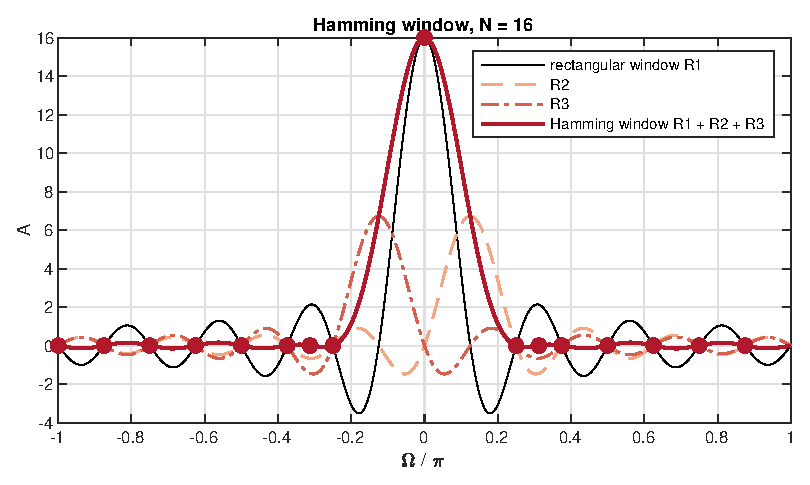
\includegraphics[]{graphics/HammingausRectWindow}
		\caption{Spectrum of Hamming window from superposition of weighted
		rectangular windows.}
		\label{HammingausRectWindow}
\end{figure}
\begin{figure}
		\centering
		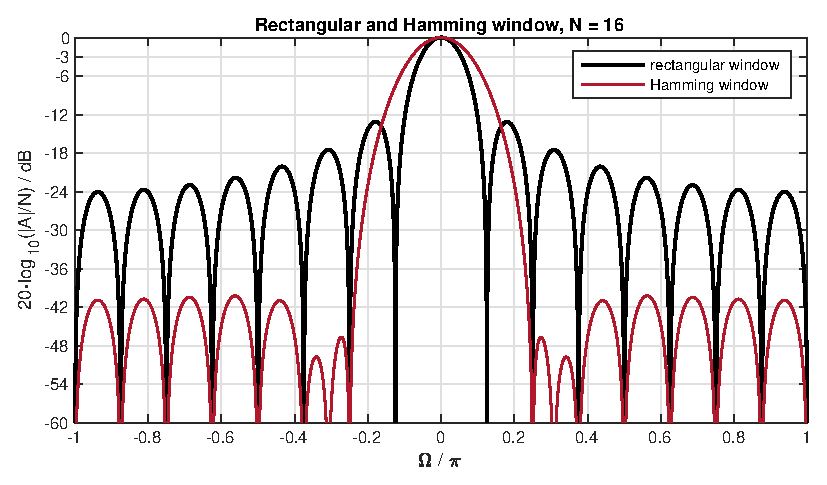
\includegraphics[]{graphics/DTFTHammingWin_log}
		\caption{Level of DTFT spectra for rectangular and Hamming window.}
		\label{DTFTHammingWin_log}
\end{figure}
\begin{figure}
		\centering
		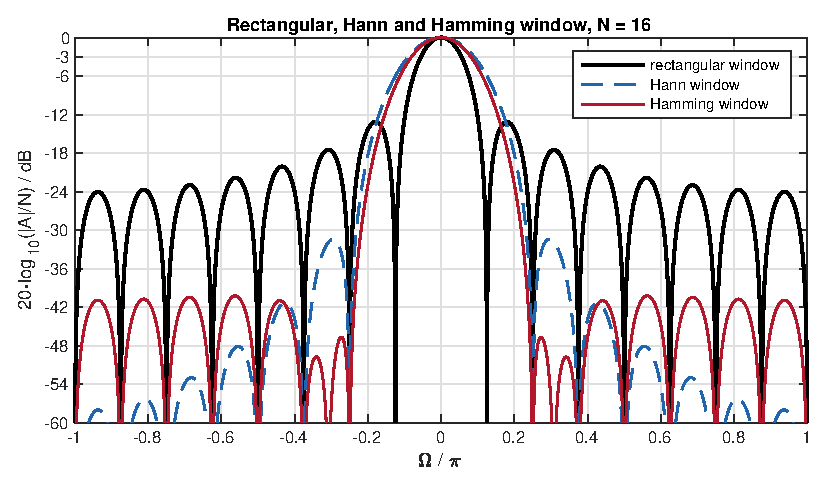
\includegraphics[]{graphics/DTFTRectHanningHammingWin_log}
		\caption{Level of DTFT spectra for rectangular, Hanning and Hamming
		window.}
		\label{DTFTRectHanningHammingWin_log}
\end{figure}
\begin{figure}
		\centering
		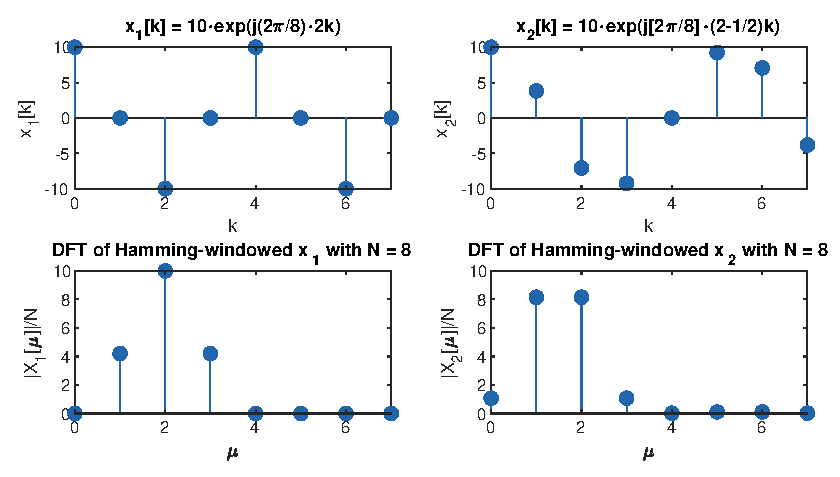
\includegraphics[]{graphics/DFTbestworstcase_HammWin}
		\caption{Hamming windowing for $N=8$, best case ($\mu=2$),
		worst case ($\mu=2-\frac{1}{2}$).}
		\label{DFTbestworstcase_HammWin}
\end{figure}

%------------------------------------------------------------------------------
\section{Exercises}

%------------------------------------------------------------------------------
\subsection*{Exercise 1: \texttt{dft}/\texttt{idft} Implementation}
\addcontentsline{toc}{subsection}{Exercise 1: \texttt{dft()}/\texttt{idft()} function}
Write Matlab/Python functions \texttt{X = my\_dft(x)} and \texttt{x = my\_idft(X)}
that calculate the DFT/IDFT-pair in eq.~\eqref{eq:DFT} and \eqref{eq:IDFT}
without using the pre-built functions \texttt{fft()} and \texttt{ifft()}
functions.
%
Check validity and performance against the built-in functions (try large $N$).
%
You might consider the matrix operation approach rather than a for-loop
implementation.

\begin{Loesung}
\textbf{Solution:} Python TBD\\\\
\red{$\rightarrow$ Matlab: \texttt{UE1\_Exercise1\_Test\_dft\_idft\_functions.m}
together with \texttt{my\_dft.m}, \texttt{my\_idft.m} and
\texttt{get\_scaledSpectrum.m}}
\end{Loesung}



% ---------------------------------------------------------------------------------
\subsection*{Exercise 2: IDFT}
\addcontentsline{toc}{subsection}{Exercise 2: IDFT}
The discrete-time signal $x[k]$
\begin{equation}
x[k]=-2\cdot\sin\left(\frac{2\pi}{4}k\right)+3\cdot\cos\left(\frac{2\pi}{4}\cdot2k\right)+1
\hspace{5mm}\text{for}\,\,0\leq k\leq3
\end{equation}
with $k\in\mathbb{Z}$ is given.
\begin{enumerate}[label=\alph*)]
	\item Calculate the resulting values of $x[k]$ for $0\leq k\leq3$.
%
	\item Show analytically that the given values of $X[\mu]$, $\mu\in\mathbb{Z}$:
	\begin{equation}
	X[\mu=0]=1, \hspace{5mm} X[\mu=1]=\im, \hspace{5mm} X[\mu=2]=3,
	\end{equation}
	are the DFT coefficients of $x[k]$ stemming from
	\begin{equation}
	X[\mu]=\frac{1}{N}\sum_{k=0}^{N-1}x[k]\cdot\e^{-\im\frac{2\pi}{N}k\mu}
	\end{equation}
	with $N=4$.
%
	The following procedure is suggested: Setup the spectral
	coefficients $X[\mu]$ in the form
	\begin{equation}
	X[\mu]=A[\mu]\cdot\e^{\im\phi[\mu]}
	\end{equation}
	and specify the missing value $X[\mu=3]$ so that the IDFT results in
	$x[k]\in\mathbb{R}$.
%
	Then calculate the IDFT as
	\begin{equation}
	x[k]=\sum_{\mu=0}^{N-1}X[\mu]\cdot\e^{\im\frac{2\pi}{N}k\mu}
	\end{equation}
	showing that this corresponds to the given signal $x[k]$.
%
	\item Plot the real and imaginary part as well as the magnitude and the phase
	of $X[\mu]$ over $\mu$.
%
	\item A DFT-based audio analyser shall exhibit a frequency resolution of
	$\Delta f=0.5$~Hz for a sampling frequency $f_s=44100$~Hz using a rectangular
	window.
%
	Determine the minimum required DFT length $N$ when only lengths $N=2^M$
	($M\in\mathbb{N}$) are allowed.
%
	What is the resulting frequency resolution then?
%
	\item Check this example with the $N=4$ DFT Matrix
	$\mathbf{W} =[\mathbf{w}_0\,\,\mathbf{w}_1\,\,\mathbf{w}_2\,\,\mathbf{w}_3]$
	for the set of linear equations
	\begin{equation}
	\mathbf{X}_{4\times1} = \mathbf{W}_{4\times4} \cdot \mathbf{x}_{4\times1}
	\end{equation}
	by interpreting the matrix multiplication as linear combination of orthogonal
	$\mathbf{w}$ vectors
	\begin{equation}
	\mathbf{X}_{4\times1} = x[0] \mathbf{w}_0
	+ x[1] \mathbf{w}_1 + x[2] \mathbf{w}_2 + x[3] \mathbf{w}_3.
	\end{equation}
\end{enumerate}

\begin{Loesung}
\textbf{Solution:}
\begin{enumerate}[label=\alph*)]
	\item \begin{align}
	x[0]&=-2\cdot\sin\left(2\pi\frac{1}{4}\cdot0\right)+3\cdot\cos\left(2\pi\frac{2}{4}\cdot0\right)+1=3+1=4\nonumber\\
	x[1]&=-2\cdot\sin\left(2\pi\frac{1}{4}\cdot1\right)+3\cdot\cos\left(2\pi\frac{2}{4}\cdot1\right)+1=-2-3+1=-4\nonumber\\
	x[2]&=-2\cdot\sin\left(2\pi\frac{1}{4}\cdot2\right)+3\cdot\cos\left(2\pi\frac{2}{4}\cdot2\right)+1=3+1=4\nonumber\\
	x[3]&=-2\cdot\sin\left(2\pi\frac{1}{4}\cdot3\right)+3\cdot\cos\left(2\pi\frac{2}{4}\cdot3\right)+1=2-3+1=0\nonumber
	\end{align}
	\item \begin{align}
	X[\mu=0]&=1=1\cdot\e^{\im\cdot0}\nonumber\\
	X[\mu=1]&=\im=1\cdot\e^{\im\frac{\pi}{2}}\nonumber\\
	X[\mu=2]&=3=3\cdot\e^{\im\cdot0}\nonumber
	\end{align}
	For $x[k]\in\mathbb{R}$ the symmetry $X[1]^*=X[3]$ holds, thus
	\begin{align}
	X[\mu=3]=1\cdot\e^{-\im\cdot\frac{\pi}{2}}.\nonumber
	\end{align}
	The IDFT is given as
	\begin{align}
	x[k]&=\sum_{\mu=0}^{N-1}X[\mu]\cdot\e^{\im\frac{2\pi}{N}k\mu}\nonumber\\
	&=\sum_{\mu=0}^{3}X[\mu]\cdot\e^{\im\frac{\pi}{2}k\mu}.\nonumber
	\end{align}
	With the spectral coefficients in the form $X[\mu]=A[\mu]\cdot\e^{\im\phi[\mu]}$ this simplifies to
	\begin{align}
	x[k]&=1\cdot\e^{\im\cdot0}\cdot\e^{\im\frac{\pi}{2}k\cdot0}+1\cdot\e^{\im\cdot\frac{\pi}{2}}\cdot\e^{\im\frac{\pi}{2}k\cdot1}+3\cdot\e^{\im\cdot0}\cdot\e^{\im\frac{\pi}{2}k\cdot2}+1\cdot\e^{-\im\cdot\frac{\pi}{2}}\cdot\e^{\im\frac{\pi}{2}k\cdot3}\nonumber\\
	&=1+\e^{\im\frac{\pi}{2}}\cdot\e^{\im\frac{\pi}{2}k}+3\cdot\e^{\im\pi k}+\e^{-\im\frac{\pi}{2}}\cdot\e^{\im\frac{3\pi}{2}k}\nonumber\\
	&=1+\e^{\im\frac{\pi}{2}}\cdot\e^{\im\frac{\pi}{2}k}+3\cdot\left(\cos(\pi k)+\underbrace{\im\cdot\sin(\pi k)}_{=0\,\,\mathrm{if}\,\,k\in\mathbb{Z}}\right)-\e^{\im\frac{\pi}{2}}\cdot\e^{-\im\frac{\pi}{2}k}\nonumber\\
	&=1+3\cdot\cos(\pi k)+\underbrace{\e^{\im\frac{\pi}{2}}}_{=\im}\cdot\left(\e^{\im\frac{\pi}{2}k}-\e^{-\im\frac{\pi}{2}k}\right).\nonumber
	\end{align}
 With Euler's identity
	\begin{equation}
	2\im\cdot\sin(x)=\e^{\im x}-\e^{-\im x}\nonumber
	\end{equation}
	one gets
	\begin{align}
	x[k]&=1+3\cdot\cos(\pi k)+\im\cdot2\im\cdot\sin\left(\frac{\pi}{2}k\right)\nonumber\\
	&=1+3\cdot\cos(\pi k)-2\cdot\sin\left(\frac{\pi}{2}k\right)\nonumber
	\end{align}
	which finally results as expected
	\begin{equation}
	x[k]=1+3\cdot\cos\left(\frac{2\pi}{4}\cdot2k\right)-2\cdot\sin\left(\frac{2\pi}{4}k\right).\nonumber
	\end{equation}
	\item \text{}
	\begin{center}%
		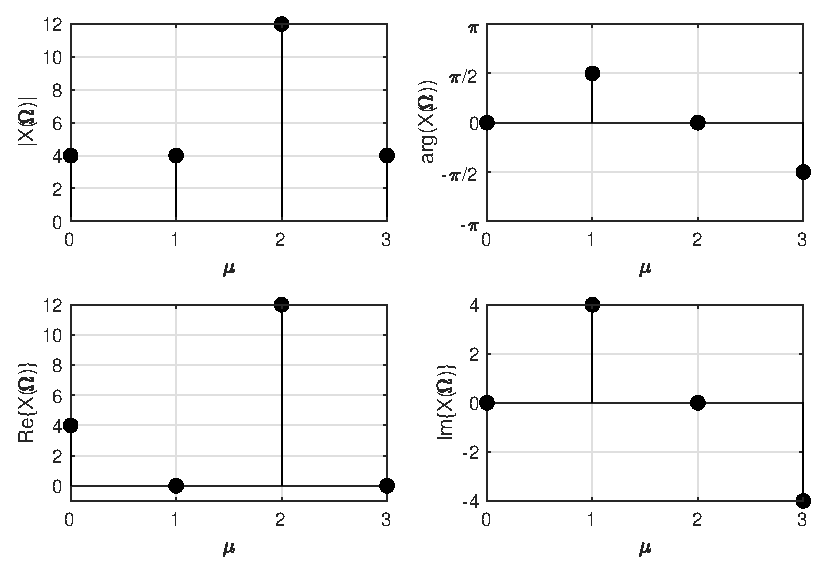
\includegraphics[width=10cm]{graphics/UE1_Exercise2_IDFT}%
		\captionof{figure}{DFT of $x[k]$ for exercise 2 c).}%
	\end{center}%
	\item \begin{align}
	\Delta f=\frac{f_s}{N}=\frac{f_s}{2^M}&\stackrel{!}{=}0.5\,\text{Hz}\nonumber\\
	M&=\left\lceil\log_{2}\left(\frac{f_s}{\Delta f}\right)\right\rceil_{\in\mathbb{N}}\nonumber\\
	&=\left\lceil\log_{2}\left(\frac{44100\,\text{Hz}}{0.5\,\text{Hz}}\right)\right\rceil_{\in\mathbb{N}}\nonumber\\
	&=\left\lceil16.4285...\right\rceil_{\in\mathbb{N}}\nonumber\\
	&=17\nonumber\\
	\Rightarrow\hspace{5mm} N&=2^M=2^{17}=131072\nonumber
	\end{align}
	The resulting frequency resolution is thus
	\begin{equation}
	\Delta f=\frac{f_s}{N}=\frac{44100\,\text{Hz}}{131072}\approx0.3365\,\text{Hz}.\nonumber
	\end{equation}
	\item
	Pay attention that this DFT is $1/N$ normalized.
	%
	Let us build the ($4\times 4$) matrix (element-wise)
	\begin{equation}
	\mathbf{W} = \mathrm{e}^{-\mathrm{j}\frac{2\pi}{4} \mathbf{A}}
	\end{equation}
	from the twiddle factor
	\begin{equation}
	W = \mathrm{e}^{-\mathrm{j}\frac{2\pi}{2}}
	\end{equation}
	and from matrix (this is an outer product)
	\begin{equation}
	\mathbf{A} =
	\begin{bmatrix}
	0\\
	1\\
	2\\
	3
	\end{bmatrix}
	\cdot
	\begin{bmatrix}
	0 & 1 & 2 & 3
	\end{bmatrix}
	=
	\mathbf{A} =
	\begin{bmatrix}
	0 & 0 & 0 & 0\\
	0 & 1 & 2 & 3\\
	0 & 2 & 4 & 6\\
	0 & 3 & 6 & 9
	\end{bmatrix}
	\end{equation}
	containing all possible products $k\,\mu$ in a suitable arrangement.
	%
	We get
	\begin{align}
	\mathbf{W} = \begin{bmatrix}
	1 & 1 & 1 & 1\\
	1 & -\mathrm{j} & -1 & \mathrm{j}\\
	1 & -1 & 1 & -1\\
	1 & \mathrm{j} & -1 & -\mathrm{j}
	\end{bmatrix},
	\mathbf{w}_1 = \begin{bmatrix}1\\1\\1\\1\end{bmatrix},
	\mathbf{w}_2 = \begin{bmatrix}1\\-\im\\-1\\\im\end{bmatrix},
	\mathbf{w}_3 = \begin{bmatrix}1\\-1\\1\\-1\end{bmatrix},
	\mathbf{w}_4 = \begin{bmatrix}1\\\im\\-1\\-\im\end{bmatrix}.
	\end{align}
	Thus,
	\begin{equation}
	4 \cdot \mathbf{X}_{4\times1} = x[0] \, \mathbf{w}_0
	+ x[1] \,\mathbf{w}_1
	+ x[2] \,\mathbf{w}_2
	+ x[3] \,\mathbf{w}_3.
	\end{equation}
	becomes
	\begin{equation}
	 4 \cdot \mathbf{X}_{4\times1} =
	 4 \cdot \begin{bmatrix}1\\\im\\3\\?\end{bmatrix}=
	 4\begin{bmatrix}1\\1\\1\\1\end{bmatrix}
  -4\begin{bmatrix}1\\-\im\\-1\\\im\end{bmatrix}
  +4\begin{bmatrix}1\\-1\\1\\-1\end{bmatrix}
	+0\begin{bmatrix}1\\\im\\-1\\-\im\end{bmatrix}
	\end{equation}
	where the ? entry is easily deduced to $-\im$.
	Think about, what this linear combination is telling you. Think of the
	DFT eigensignals (rows) and index of DFT eigenfrequencies (columns) and the
	signal samples acting as weights.
\end{enumerate}
\end{Loesung}



%------------------------------------------------------------------------------
\subsection*{Exercise 3: DFT analysis using a rectangular window}
\addcontentsline{toc}{subsection}{Exercise 3: DFT Analysis Using a Rectangular Window}
A sine signal $x[k]=\cos(\Omega k)$ with $\Omega=2\cdot\frac{2\pi}{N}$, $N=8$,
$0\leq k \leq N-1$ is to be analysed with the DFT eq.~\eqref{eq:DFT} assuming a
sampling frequency of $f_s=48$~kHz.
%
\begin{enumerate}[label=\alph*)]
	\item Calculate the spectrum $X[\mu]$ of $x[k]$ and visualise the real and
	imaginary part as well as the magnitude and the phase of $X[\mu]$ over
	$0\leq\mu\leq N-1$.
%
	\item Check the expected symmetries.
%
	\item Implement the interpolation of eq.~\eqref{eq:DTFT_Interpolation_psinc}
	and visualise this over $\mu$, $\Omega$ as well as $f$ as a magnitude
	spectrum together with $|X[\mu]|$.
%
	\item Repeat the steps a) to c) for $N=9$. What is different?
%
	\item Repeat the steps a) to d) for $\Omega=2.5\cdot\frac{2\pi}{N}$.
	What is different now?
\end{enumerate}

\begin{Loesung}
\textbf{Solution:} Python TBD\\\\
\red{$\rightarrow$ Matlab: \texttt{UE1\_Exercise3\_DFT\_analysis.m}
together with \texttt{interpolate\_DFT.m}}
\end{Loesung}



% ---------------------------------------------------------------------------------
\subsection*{Exercise 4: DFT of an Impulse Response}
\addcontentsline{toc}{subsection}{Exercise 4: DFT of an impulse response}
The finite length impulse response (FIR filter) $h[k]$ of an LTI system is given
as
%
\begin{equation}
h[k]=\frac{1}{8}\cdot\left(11\cdot\delta[k]-5\cdot\delta[k-1]+7\cdot\delta[k-2]-9\cdot\delta[k-3]\right)
\end{equation}
%
\begin{enumerate}[label=\alph*)]
	\item Calculate the DFT analytically
%
	\begin{equation}
	H[\mu]=\sum_{k=0}^{N-1}h[k]\cdot\e^{-\im\frac{2\pi}{N}k\mu}
	\end{equation}
	for $N=4$ and $0\leq k\leq N-1$.
	The DFT spectrum corresponds to the transfer function of the system.
%
	\item Calculate the magnitude $|H[\mu]|$ and the phase response $\arg(H[\mu])$
	for $0\leq\mu\leq 3$. State the magnitude as level in dB and the phase in
	degrees.
%
	\item The frequency resolution is assumed to be $\Delta f=500\,\text{Hz}$.
	Sketch the DFT line spectrum and the interpolated DTFT spectrum of the
	magnitude $|H[\mu]|$ in dB and the phase $\arg(H[\mu])$ in degrees over the
	frequency axis from $0\,\text{Hz}\leq f\leq4000\,\text{Hz}$.
	Estimate the sampling frequency $f_s$ from the known parameters and information.
	What filter characteristic is realised with this impulse response?
\end{enumerate}

\begin{Loesung}
\textbf{Solution:}
\begin{enumerate}[label=\alph*)]
	\item For $N=4$, the DFT is
	\begin{equation}
	H[\mu]=\sum_{k=0}^{3}h[k]\e^{-\im\frac{2\pi}{4}\mu k}=\sum_{k=0}^{3}h[k]\e^{-\im\frac{\pi}{2}\mu k}\nonumber
	\end{equation}
	with the twiddle factors
	\begin{equation}
	W_4^{\mu k}=\e^{-\im\frac{\pi}{2}\mu k}\nonumber.
	\end{equation}
	Again, the DFT matrix is built:
	\begin{center}
		\begin{tabular}{|c|c|c|c|c|}
		\hline
		$W_4^{\mu k}$ & $k=0$ & $k=1$ & $k=2$ & $k=3$\\\hline
		$\mu=0$ & $1$ & $1$ & $1$ & $1$\\\hline
		$\mu=1$ & $1$ & $-\im$ & $-1$ & $\im$\\\hline
		$\mu=2$ & $1$ & $-1$ & $1$ & $-1$\\\hline
		$\mu=3$ & $1$ & $\im$ & $-1$ & $-\im$\\\hline
		\end{tabular}
	\end{center}
	Hence, for $H[\mu]$ follows (this time using the row times column matrix
	multiplication approach written in detail)
	\begin{align}
	H[0]&=\sum_{k=0}^{3} W_4^{0\cdot k} \cdot h[k]=\left(\frac{11}{8}\cdot1\right)+\left(\frac{-5}{8}\cdot1\right)+\left(\frac{7}{8}\cdot1\right)+\left(\frac{-9}{8}\cdot1\right)=\frac{4}{8}=\frac{1}{2}\nonumber\\
	H[1]&=\sum_{k=0}^{3} W_4^{1\cdot k} \cdot h[k]=\left(\frac{11}{8}\cdot1\right)+\left(\frac{-5}{8}\cdot(-\im)\right)+\left(\frac{7}{8}\cdot(-1)\right)+\left(\frac{-9}{8}\cdot\im\right)=\frac{4}{8}-\im\frac{4}{8}=\frac{1}{2}-\im\frac{1}{2}\nonumber\\
	H[2]&=\sum_{k=0}^{3} W_4^{2\cdot k} \cdot h[k]=\left(\frac{11}{8}\cdot1\right)+\left(\frac{-5}{8}\cdot(-1)\right)+\left(\frac{7}{8}\cdot1\right)+\left(\frac{-9}{8}\cdot(-1)\right)=\frac{32}{8}=4\nonumber\\
	H[3]&=\sum_{k=0}^{3} W_4^{3\cdot k} \cdot h[k]=\left(\frac{11}{8}\cdot1\right)+\left(\frac{-5}{8}\cdot\im\right)+\left(\frac{7}{8}\cdot(-1)\right)+\left(\frac{-9}{8}\cdot(-\im)\right)=\frac{4}{8}+\im\frac{4}{8}=\frac{1}{2}+\im\frac{1}{2}\nonumber
	\end{align}
	\item \begin{align}
	|H[0]|&=\frac{1}{2} \hspace{5mm}\longrightarrow\hspace{5mm} 20\log_{10}\left(\frac{1}{2}\right)=-6.02\,\text{dB}\nonumber\\
	|H[1]|&=\sqrt{\frac{1}{2^2}+\frac{1}{2^2}}=\frac{1}{\sqrt{2}} \hspace{5mm}\longrightarrow\hspace{5mm} 20\log_{10}\left(\frac{1}{\sqrt{2}}\right)=-3.01\,\text{dB}\nonumber\\
	|H[2]|&=4 \hspace{5mm}\longrightarrow\hspace{5mm} 20\log_{10}(4)=12.04\,\text{dB}\nonumber\\
	|H[3]|&=\sqrt{\frac{1}{2^2}+\frac{1}{2^2}}=\frac{1}{\sqrt{2}} \hspace{5mm}\longrightarrow\hspace{5mm} 20\log_{10}\left(\frac{1}{\sqrt{2}}\right)=-3.01\,\text{dB}\nonumber\\
	\arg(H[0])&=0\nonumber\\
	\arg(H[1])&=\arctan\left(\frac{-\frac{1}{2}}{\frac{1}{2}}\right)=-0.7854\,\hat{=}\,-45^{\circ}\nonumber\\
	\arg(H[2])&=0\nonumber\\
	\arg(H[3])&=\arctan\left(\frac{\frac{1}{2}}{\frac{1}{2}}\right)=0.7854\,\hat{=}\,45^{\circ}\nonumber
	\end{align}
	\item \text{}
	\begin{center}%
		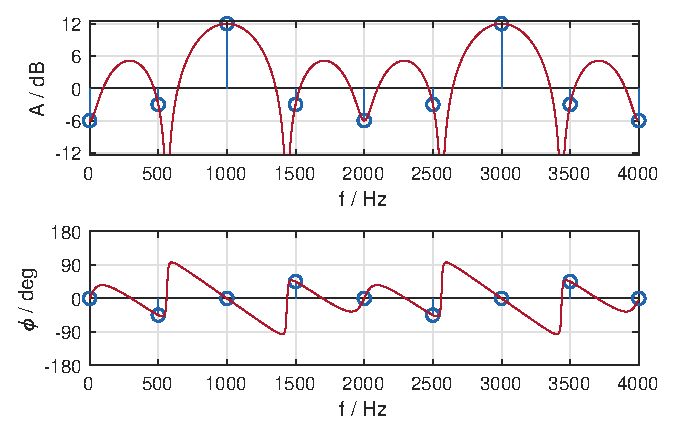
\includegraphics[]{graphics/UE1_Exercise4_Spectrum}%
		\captionof{figure}{DFT and interpolated DTFT spectrum for $h[k]$}%
	\end{center}%
	\underline{sampling frequency:} $\Delta f=\frac{f_s}{N}\,\,\Leftrightarrow\,\,f_s=\Delta f\cdot N=500\,\text{Hz}\cdot4=2000\,\text{Hz}$\\\\
	\underline{filter characteristic:} highpass filter, -3~dB corner frequency at
	about 790~Hz, relative sidelobe level about -7~dB, notch at about 560~Hz,
	12~dB gain at $\frac{f_s}{2}$
\end{enumerate}
\end{Loesung}



% ---------------------------------------------------------------------------------
\subsection*{Exercise 5: DFT Parameterisation}
\addcontentsline{toc}{subsection}{Exercise 5: DFT parameterisation}
A composite signal
$x[k]=A_1\cdot\e^{\im(\Omega_1 k+\phi_1)}+A_2\cdot\e^{\im(\Omega_2 k+\phi_2)}$
with the known frequencies $\Omega_1=\frac{1}{30}\pi$ und $\Omega_2=\frac{1}{4}\pi$
but unknown amplitudes and phase relation is given.
%
\begin{enumerate}[label=\alph*)]
	\item What DFT length $N$ must be set up so that the exact amplitude and
	phase values for both frequencies $\Omega_1$ and $\Omega_2$ can be determined
	for a rectangularly windowed signal (i.e. no leakage occurs)?
%
	\item In which bins are the frequencies $\Omega_1$ and $\Omega_2$ then found?
%
	\item What amplitude deviation occurs when analysing the signal
	$x[k]=\e^{\im\Omega_3k}$ with $\Omega_3=\frac{30.5}{60}\pi$?
\end{enumerate}

\begin{Loesung}
\textbf{Solution:}
\begin{enumerate}[label=\alph*)]
	\item DFT eigenfrequencies: $\Omega_\text{DFT}=\frac{2\pi}{N}\mu$\\\\
	$\Omega_1$ and $\Omega_2$ must be DFT eigenfrequencies:
%
	\begin{align}
	\Omega_1&=\frac{\pi}{30}=\frac{2\pi}{N}\mu \hspace{5mm}\Leftrightarrow\hspace{5mm} N=60\cdot\mu\nonumber\\
	\Omega_2&=\frac{\pi}{4}=\frac{2\pi}{N}\mu \hspace{5mm}\Leftrightarrow\hspace{5mm} N=8\cdot\mu\nonumber
	\end{align}
%
	Both conditions together can be fulfilled from $N=120$ (or multiples thereof).
%
	\item \begin{align}
	\mu_1&=\Omega_1\cdot\frac{N}{2\pi}=\frac{\pi}{30}\cdot\frac{120}{2\pi}=2, \hspace{5mm}\text{i.e. the 3rd bin}\nonumber\\
	\mu_2&=\Omega_2\cdot\frac{N}{2\pi}=\frac{\pi}{4}\cdot\frac{120}{2\pi}=15, \hspace{5mm}\text{i.e. the 16th bin}\nonumber
	\end{align}
%
	\item The discrete angular frequency $\Omega_3=\frac{30.5}{60}\pi$ can be
	expressed in terms of multiples of the first DFT eigenfrequency
	$\frac{2\pi}{N}$ as
%
	\begin{equation}
	\Omega_3=n\cdot\frac{2\pi}{N} \hspace{5mm}\leftrightarrow\hspace{5mm} n=\Omega_3\cdot\frac{N}{2\pi}=\frac{30.5}{60}\pi\cdot\frac{120}{2\pi}=30.5\nonumber
	\end{equation}
%
	so that
%
	\begin{equation}
	\Omega_3=30.5\cdot\frac{2\pi}{N}.\nonumber
	\end{equation}
%
	The frequency $\Omega_3$ is not a DFT eigenfrequency as it is not an integer
	multiple of the first DFT eigenfrequency, but is located in the middle between
	bins 31 and 32 (for $\mu=30$ and $\mu=31$ counting from $\mu=0$).
%
	The neighbouring bins are the bins that can give the best information about
	the amplitude of the true signal.
%
	The spectral values at the neighbouring bins can be calculated by the DFT of
	a complex exponential (see formularies)
%
	\begin{equation}
	\e^{\im\Omega_3 k} \hspace{5mm}\laplace\hspace{5mm} \e^{\im\frac{\left(\Omega_3-\frac{2\pi}{N}\mu\right)(N-1)}{2}}\cdot\frac{\sin\left(N\frac{\Omega_3-\frac{2\pi}{N}\mu}{2}\right)}{\sin\left(\frac{\Omega_3-\mu\frac{2\pi}{N}}{2}\right)}.\nonumber
	\end{equation}
%
	At $\mu=30$, the amplitude is
%
	\begin{align}
	|X[\mu=30]|&=\left|\e^{\im\frac{\left(\Omega_3-\frac{2\pi}{N}\mu\right)(N-1)}{2}}\cdot\frac{\sin\left(N\frac{\Omega_3-\frac{2\pi}{N}\mu}{2}\right)}{\sin\left(\frac{\Omega_3-\frac{2\pi}{N}\mu}{2}\right)}\right|\nonumber\\
	&=\frac{\sin\left(N\frac{\Omega_3-\frac{2\pi}{N}\mu}{2}\right)}{\sin\left(\frac{\Omega_3-\frac{2\pi}{N}\mu}{2}\right)}\nonumber\\
	&=\frac{\sin\left(N\frac{30.5\cdot\frac{2\pi}{N}-30\cdot\frac{2\pi}{N}}{2}\right)}{\sin\left(\frac{30.5\cdot\frac{2\pi}{N}-30\cdot\frac{2\pi}{N}}{2}\right)}\nonumber\\
	&=\frac{\sin\left(N\frac{\frac{1}{2}\cdot\frac{2\pi}{N}}{2}\right)}{\sin\left(\frac{\frac{1}{2}\cdot\frac{2\pi}{N}}{2}\right)}\nonumber\\
	&=\frac{\sin\left(\frac{\pi}{2}\right)}{\sin\left(\frac{\pi}{2N}\right)}\nonumber\\
	&=\frac{1}{\sin\left(\frac{\pi}{240}\right)}\nonumber\\
	&\approx76.3966.\nonumber
	\end{align}
%
	At $\mu=31$, the amplitude is
%
	\begin{align}
	|X[\mu=31]|&=\frac{\sin\left(N\frac{30.5\cdot\frac{2\pi}{N}-31\cdot\frac{2\pi}{N}}{2}\right)}{\sin\left(\frac{30.5\cdot\frac{2\pi}{N}-31\cdot\frac{2\pi}{N}}{2}\right)}\nonumber\\
	&=\frac{\sin\left(-\frac{\pi}{2}\right)}{\sin\left(-\frac{\pi}{2N}\right)}\nonumber\\
	&\approx76.3966.\nonumber
	\end{align}
%
	If the frequency of the complex exponential had been exactly at a DFT
	eigenfrequency, e.g. at $\mu=31$, the DFT spectrum would have contained the
	true amplitude of the signal.
	The rule of L'Hospital is needed to to calculate this amplitude value:
%
	\begin{align}
	&\lim_{\Omega_3\to31\cdot\frac{2\pi}{N}}\frac{\sin\left(N\frac{\Omega_3-\frac{2\pi}{N}31}{2}\right)}{\sin\left(\frac{\Omega_3-\frac{2\pi}{N}31}{2}\right)}\nonumber\\
	=&\lim_{\Omega_3\to31\cdot\frac{2\pi}{N}}\frac{\cos\left(N\frac{\Omega_3-\frac{2\pi}{N}31}{2}\right)\cdot\frac{N}{2}}{\cos\left(\frac{\Omega_3-\frac{2\pi}{N}31}{2}\right)\cdot\frac{1}{2}}\nonumber\\
	=&\frac{\cos0}{\cos0}\cdot N\nonumber\\
	=&N\nonumber\\
	=&120\nonumber.
	\end{align}
%
	The error is thus
	\begin{equation}
	20\cdot\log_{10}\left(\frac{76.3966}{120}\right)=-3.9221\,\text{dB},\nonumber
	\end{equation}
	i.e. the magnitude is underestimated.
	The case when the signal frequency lies exactly in middle between two DFT
	eigenfrequencies is the worst case scenario, in \cite{Harris1978}
	termed "worst case process loss".
\end{enumerate}
\end{Loesung}

%------------------------------------------------------------------------------
\bibliographystyle{Schultz_PHD}
%\bibliographystyle{IEEEtran}
\bibliography{literature}
\end{document}
